\documentclass[runningheads,a4paper]{llncs}

\usepackage{amsmath}
\usepackage{amssymb}
\usepackage{color}
\usepackage{float}
\usepackage{hyperref}
\usepackage{pgfplots}
\usepackage{rotating}
\usepackage{tabularx}
\usepackage{textcomp}
\usepackage{url}
\newcommand{\keywords}[1]{\par\addvspace\baselineskip
\noindent\keywordname\enspace\ignorespaces#1}
\pgfplotsset{compat=1.11}
\setcounter{tocdepth}{3}
\setcounter{secnumdepth}{3}
\usetikzlibrary{spy}
\usetikzlibrary{pgfplots.colormaps}
\usepgfplotslibrary{external}
\tikzexternalize
\def\arraystretch{1.2}

\begin{document}
    \graphicspath{{../img/}}
    \mainmatter
    \title{A Sliding Window Filter for Time Series Streams}
    \subtitle{Bachelor thesis\\
    \textnormal{\small{Supervisor: Stephan Spiegel}}}
    \titlerunning{A Sliding Window Filter for Time Series Streams}
    \author{Gordon Lesti\\
    313249\\
    Course of studies: Bachelor of Computer Science\\
    gordon.lesti@campus.tu-berlin.de\\}
    \authorrunning{Gordon Lesti}
    \institute{Technische Universit\"at Berlin\\
    Fakult\"at IV Elektrotechnik und Informatik\\
    Fachgebiet AOT\\
    Prof. Dr. Sahin Albayrak\\
    \url{http://www.aot.tu-berlin.de/}}
    \toctitle{A Sliding Window Filter for Time Series Streams}
    \tocauthor{Gordon Lesti}
    \pagenumbering{Roman}
    \let\oldaddcontentsline\addcontentsline
    \def\addcontentsline#1#2#3{}
    \maketitle
    \def\addcontentsline#1#2#3{\oldaddcontentsline{#1}{#2}{#3}}

    \renewcommand{\abstractname}{\normalsize Abstract.}
\begin{abstract} \addcontentsline{toc}{section}{Abstract}
    \normalsize
    A lot of devices with various sensors in the modern humans everyday life are producing constantly a diverse kind of
    data. Obvious examples are smartphones, wearable devices like smartwatches and fitness tracker braclets. A
    considerable part of the produced data comes continuously and can be interpreted as time series streams. For example
    acceleration or vitality data. A real time evaluation of the time series stream presupposes possibly a constantly
    running 1-Nearest-Neighbour (1NN) classification on the most recent time series window with a distance measure like
    Dynamic Time Warping (DTW). The limited resources of wearable devices or microcontrollers forces to a frugal usage
    of memory and running time.

    This bachelor thesis explains the approach of a filter with linear complexity for time series ahead of a 1NN-DTW.
    The added value of a filter with cost efficient running time is to reduce the execution of a cost intensive 1NN-DTW
    in the case of unclassifiable time series windows. On results of an experimental example with gesture detection via
    acceleration data will be shown that filters can reduce the execution of 1NN-DTW without loss of accuracy.
    \keywords{Time Series, Distance Measures, Classification}\\
\end{abstract}

    \clearpage
    \section*{Eidesstattliche Erkl\"arung}
Hiermit erkl\"are ich, dass ich die vorliegende Arbeit selbstst\"andig und eigenh\"andig sowie ohne unerlaubte fremde
Hilfe und ausschlie{\ss}lich unter Verwendung der aufgef\"uhrten Quellen und Hilfsmittel angefertigt habe.\\\\
Die selbstst\"andige und eigenst\"andige Anfertigung versichert an Eides statt:\\\\
Berlin, den\\\\\\
..................................................\\
\textit{Unterschrift}

    \tableofcontents
    \clearpage
    \pagenumbering{arabic}
    \section{Introduction} \label{introduction}
The scenario used for this thesis is an application which constantly receives data in form of a time series stream from
one or more sensors. The application itself does not have a general interest in a long term evaluation of the data. Only
the most recent time series window has to be classified in the evaluation. The result of the evaluation can be stored or
processed by an other application, the time series window moves on and has to be evaluated again. This process is
continuously repeated with every times series window being readable only once. Dynamic Time Warping (DTW) in combination
with a 1-Nearest-Neighbour (1NN) classification for the evaluation is an obvious approach for such a scenario. The
disadvantage is that this approach is computationally too demanding for many realtime applications \cite{xi2006fast}.
This disadvantage becomes even more tragic under the assumption that perhaps a large amout of incoming time series
windows is unclassifiable due to a too large distance to the nearest neighbour.

This bachelor thesis explains the approach of a sliding window filter for time series ahead of the 1NN in combination
with DTW (1NN-DTW) to reduce the execution of 1NN-DTW on unclassifiable time series windows. The condition for such a
filter is linear complexity. Furthermore the combination of the filter ahead of the 1NN-DTW should perform with a
similar accuracy as 1NN-DTW on its own.

An experiment that simulates an above described scenario was carried out to expose the additional benefit of a filter
ahead of 1NN-DTW under the given conditions.%TODO double of

The bachelor thesis is organized as follows. Section \ref{background_and_notation} will explain the sliding window
technique and basics around time series similarity measures that are used in this bachelor thesis. Furthermore
the sliding window filter is described at the end of the same section. The description of the experiment and the
evaluation of the results are contained in section \ref{experiment}. Conclusions are offered and future work
is suggested in section \ref{conclusion_and_future_work}.

    \section{Background and Notation} \label{background_and_notation}
A time series $Q$ with the length $l$ over the domain set $\mathbb{U}$ is a sequence of data points
$Q = (q_1, q_2, \dots, q_i, \dots, q_l)$ with $q_i \in \mathbb{U}$. On the set $\mathbb{U}$ exists a distance measure
function $D$ with $D: \mathbb{U} \times \mathbb{U} \to \mathbb{R}$. A common assumption for time series is that the
containing data points are elements of the integer numbers $\mathbb{Z}$ or the real numbers $\mathbb{R}$. The distance
measure function on these common domains is just the absolute value of the difference of two elements. A fundamental
prerequisite for similarity measures on time series is often the distance measure function $D$ on the set
$\mathbb{U}$. Table~\ref{tab:notation} explains the basic notation that is used in this bachelor thesis.

\begin{table}
    \begin{center}
        \begin{tabularx}{\textwidth}{c X l}
            \textbf{Symbol} \qquad & \textbf{Description} & \qquad \textbf{Section}\\
            \hline
            $\mathbb{U}$ & a set containing all items of a domain & \qquad \ref{background_and_notation}\\
            $D$ & a distance measure function on $\mathbb{U}$ with $D: \mathbb{U} \times \mathbb{U} \to \mathbb{R}$
                & \qquad \ref{background_and_notation}\\
            $ADD$ & a summing function on $\mathbb{U}$ with $ADD: \mathbb{U} \times \mathbb{U} \to \mathbb{U}$
                & \qquad \ref{background_and_notation}\\
            $SMULT$ & a scalar multiplication function with $SMULT: \mathbb{R} \times \mathbb{U} \to \mathbb{U}$
                & \qquad \ref{background_and_notation}\\
            $Q$ & a time series over the set $\mathbb{U}$ of size $l$ with
                $Q = (q_1, q_2, \dots, q_i, \dots, q_l), q_i \in \mathbb{U}$ & \qquad \ref{background_and_notation}\\
            ED & Euclidean Distance, a similarity measure for time series & \qquad \ref{euclidean_distance}\\
            DTW & Dynamic Time Warping, a similarity measure for time series & \qquad \ref{dynamic_time_warping}\\
            CID & Complexity-Invariant Distance, a similarity measure for time series
                & \qquad \ref{complexity-invariant_distance_measure}\\
            CF & Complexity Correction Factor & \qquad \ref{complexity-invariant_distance_measure}\\
            CE & Complexity Estimate & \qquad \ref{complexity-invariant_distance_measure}\\
            CIDDTW & Complexity-Invariant Dynamic Time Warping
                & \qquad \ref{complexity-invariant_dynamic_time_warping}\\
            ACE & Avergae Complexity Estimate & \qquad \ref{sliding_window_filter_measures}\\
            VAR & Sample Variance & \qquad \ref{sliding_window_filter_measures}\\
        \end{tabularx}
    \end{center}
    \caption{Basic notation.}
	\label{tab:notation}
\end{table}

\subsection{Euclidean Distance}
The Euclidean Distance (ED) is the most straightforward similarity measure for time series \cite{ding2008querying}.
Given are two time series $Q = (q_1, q_2, \dots, q_i, \dots, q_l)$, $C = (c_1, c_2, \dots, c_j, \dots, c_l)$ with the
same length $l$ over the domain set $\mathbb{U}$ and a distance measure function $D$ with
$D: \mathbb{U} \times \mathbb{U} \to \mathbb{R}$. The ED between those two time series can be calculated with the
following formula.
\begin{center}
    $ED(Q, C) = \sqrt[2]{\sum \limits_{i=1}^{l} D(q_i, c_i)^2}$
\end{center}

\begin{figure}[H]
    \begin{center}
        \begin{tikzpicture}
            \begin{axis}[
                xlabel=time,
                ylabel=acceleration,
                width=\textwidth,
                height=\axisdefaultheight]
                \addplot[blue, mark=none] table[x=t, y=q] {background_and_notation/euclidean_distance/timeseries.dat};
                \addlegendentry{Q}
                \addplot[red, mark=none] table[x=t, y=c] {background_and_notation/euclidean_distance/timeseries.dat};
                \addlegendentry{C}
                \addplot[gray, quiver={v=\thisrow{v}}] table[x=t, y=q] {background_and_notation/euclidean_distance/timeseries.dat};
            \end{axis}
        \end{tikzpicture}
    \end{center}
    \caption{Two time series $Q$ and $C$ containing recorded data from one acceleration sensor. The square root of the
    sum of the gray distance lines illustrate the Euclidean distance between the two time series.}
    \label{fig:euclideandistance}
\end{figure}

An advantage of ED is the linear time and space complexity of $\mathcal{O}(l)$ to calculate the similarity between two
time series. The algorithm itself has even only a space complexity of $\mathcal{O}(1)$ if the space of the input time
series is ignored. Comparing two time series of different length with the ED presupposes to transform the time series
to the same length. That can be achieved by stretch the smaller time series for example. Figure
\ref{fig:euclideandistance} illustrates the Euclidean Distance between a time series $Q$ and $C$ that contain recorded
data from one acceleration sensor.

\subsubsection{Dynamic Time Warping}
Dynamic time warping or just shorten DTW is a well known algorithm for pattern detection in time series
\cite{berndt1994using}. The following short description of the algorithm will only focus on the distance calculation and
not on the backtracking. The warping path as result of the backtracking is irrelevant for the aim of this bachelor
thesis.

Given are a time series $S$ of size $n$ and a time series $T$ of size $m$ over the set $U$. Furthermore is given a
distance measure function $D$ on set $\mathbb{U}$ with $D: \mathbb{U} \times \mathbb{U} \to \mathbb{R}$. DTW creates a
$n \times m$ grid $M$ with the the following rule.
\begin{center} \[ M_{i, j} = \begin{cases}
    D(s_i,t_j) & \text{if } i = 1 \wedge j = 1\\
    M_{i,j-1} + D(s_i,t_j) & \text{if } i = 1 \wedge j \neq 1\\
    M_{i-1,j} + D(s_i,t_j) & \text{if } i \neq 1 \wedge j = 1\\
    min(M_{i-1,j}, M_{i-1,j-1}, M_{i,j-1}) + D(s_i,t_j) & \text{if } i \neq 1 \wedge j \neq 1
\end{cases} \] \end{center}
The resulting distance between the two given time series is the entry $M_{n,m}$ of the grid.
\begin{center}
    $DTW(S, T) = M_{n,m}$
\end{center}

\subsection{Complexity-Invariant Distance Measure} \label{complexity-invariant_distance_measure}
The Complexity-Invariant Distance measure \cite{batista2011complexity} (CID) is a distance measure for time
series. It is composed of the ED and a Complexity Correction Factor (CF).

% Given are a time series $S$ of size $n$ and a time series $T$ of size $m$ over the set $\mathbb{U}$. Furthermore is
% $n = m$ and a distance measure function $D$ on the set $\mathbb{U}$ with
% $D: \mathbb{U} \times \mathbb{U} \to \mathbb{R}$ is given.
% \begin{center}
%     $CID(S, T) = ED(S, T) \times CF(S, T)$
% \end{center}
% with complexity correction factor
% \begin{center}
%     $CF(S, T) = \frac{max(CE(S), CE(T))}{min(CE(S), CE(T))}$
% \end{center}
% $CE$ is a complexity estimate of a time series and a possible implementation can be
% \begin{center}
%     $CE(S) = \sqrt[2]{\sum \limits_{i=1}^{n-1} D(s_i, s_{i + 1})^2}$
% \end{center}

\subsubsection{Time Series Normalization}

\begin{frame}{Time Series Normalization}
    \begin{itemize}
        \item z-normalization or Z-scoring time series is common prior DTW calculation \cite{ding2008querying}
        
        \item Two different time series normalizations $\eta$ and $\eta '$ from \cite{das1998rule}
    \end{itemize}
\end{frame}

\begin{frame}{Time Series Normalization}{Calculation}
    \begin{block}{Given}
        \begin{itemize}
            \item A domain set $\mathbb{U}$
            
            \item A distance measure function $d$ with $d: \mathbb{U} \times \mathbb{U} \to \mathbb{R}$
            
        \end{itemize}
    \end{block}
    \begin{block}{Input}
        \begin{itemize}
            \item A time series $Q = (q_1, q_2, \dots, q_i, \dots, q_l)$ with length $l$ over the domain set
                $\mathbb{U}$
        \end{itemize}
    \end{block}
\end{frame}

\begin{frame}{Time Series Normalization $\eta$}{Calculation}
    \begin{block}{Calculation}
        \begin{itemize}
            \item Every data point $q$ of $Q$ will be transformed by $\eta$
            
            \item $\eta (q) = q -\bar{q}$
            
        \end{itemize}
    \end{block}
    \begin{block}{Mean of $Q$}
        \begin{itemize}
            \item $\bar{q} = \frac{1}{l} \sum \limits_{i=1}^{l} q_i$
        \end{itemize}
    \end{block}
\end{frame}

\begin{frame}<handout:0>{Time Series Normalization $\eta$}{Example}
    \begin{center}
        \resizebox {\textwidth} {!} {
            \begin{tabular}{cc}
                \resizebox* {!} {0.3\textwidth} {
                    \begin{tikzpicture}
                        \begin{axis}[
                            xmin=0,
                            xmax=47,
                            xlabel=time,
                            ylabel=acceleration,
                            width=\axisdefaultwidth,
                            height=0.7*\axisdefaultheight,
                            reverse legend,
                            legend pos=south east]
                            \addplot[red, thick, mark=none] table {../data/fig/dynamictimewarping/q.dat};
                            \addlegendentry{Q}
                            \addplot[blue, thick, mark=none] table {../data/fig/dynamictimewarping/c.dat};
                            \addlegendentry{C}
                        \end{axis}
                    \end{tikzpicture}
                } & \quad
                \resizebox* {!} {0.3\textwidth} {
                    \begin{tabular}[b]{ll}
                        \begin{turn}{90}
                            \begin{tikzpicture}
                                \begin{axis}[
                                    xmin=0,
                                    xmax=47,
                                    ymin=-100,
                                    ymax=0,
                                    hide x axis,
                                    hide y axis,
                                    width=\axisdefaultwidth,
                                    height=0.7*\axisdefaultheight]
                                    \addplot[red, ultra thick, mark=none] table {../data/fig/dynamictimewarping/q.dat};
                                \end{axis}
                            \end{tikzpicture}
                        \end{turn} \hspace*{3em} &
                        \begin{tikzpicture}
                            \begin{axis}[
                                enlargelimits=false,
                                ymin=0,
                                ymax=47,
                                hide x axis,
                                hide y axis,
                                width=\axisdefaultwidth,
                                height=\axisdefaultwidth,
                                colorbar,
                                colormap/viridis high res]
                                \addplot[matrix plot*,
                                    mesh/cols=48,
                                    point meta=explicit] table[meta=C] {../data/fig/dynamictimewarping/matrix.dat};
                            \end{axis}
                        \end{tikzpicture} \\
                        &
                        \\[1em]
                        &
                        \begin{tikzpicture}
                            \begin{axis}[
                                xmin=0,
                                xmax=47,
                                ymin=-100,
                                ymax=0,
                                hide x axis,
                                hide y axis,
                                width=\axisdefaultwidth,
                                height=0.7*\axisdefaultheight]
                                \addplot[blue, ultra thick, mark=none] table {../data/fig/dynamictimewarping/c.dat};
                            \end{axis}
                        \end{tikzpicture}
                    \end{tabular}
                }
            \end{tabular}
        }
    \end{center}
\end{frame}

\begin{frame}<handout:0>{Time Series Normalization $\eta$}{Example}
    \begin{center}
        \resizebox {\textwidth} {!} {
            \begin{tabular}{cc}
                \resizebox* {!} {0.3\textwidth} {
                    \begin{tikzpicture}
                        \begin{axis}[
                            xmin=0,
                            xmax=47,
                            xlabel=time,
                            ylabel=acceleration,
                            width=\axisdefaultwidth,
                            height=0.7*\axisdefaultheight,
                            reverse legend,
                            legend pos=south east]
                            \addplot[red, thick, mark=none] table {../data/fig/norm1/q.dat};
                            \addlegendentry{Q}
                            \addplot[blue, thick, mark=none] table {../data/fig/norm1/c.dat};
                            \addlegendentry{C}
                        \end{axis}
                    \end{tikzpicture}
                } & \quad
                \resizebox* {!} {0.3\textwidth} {
                    \begin{tabular}[b]{ll}
                        \begin{turn}{90}
                            \begin{tikzpicture}
                                \begin{axis}[
                                    xmin=0,
                                    xmax=47,
                                    ymin=-40,
                                    ymax=40,
                                    hide x axis,
                                    hide y axis,
                                    width=\axisdefaultwidth,
                                    height=0.7*\axisdefaultheight]
                                    \addplot[red, ultra thick, mark=none] table {../data/fig/norm1/q.dat};
                                \end{axis}
                            \end{tikzpicture}
                        \end{turn} \hspace*{3em} &
                        \begin{tikzpicture}
                            \begin{axis}[
                                enlargelimits=false,
                                ymin=0,
                                ymax=47,
                                hide x axis,
                                hide y axis,
                                width=\axisdefaultwidth,
                                height=\axisdefaultwidth,
                                colorbar,
                                colormap/viridis high res]
                                \addplot[matrix plot*,
                                    mesh/cols=48,
                                    point meta=explicit] table[meta=C] {../data/fig/norm1/matrix.dat};
                            \end{axis}
                        \end{tikzpicture}\\
                        &
                        \\[1em]
                        &
                        \begin{tikzpicture}
                            \begin{axis}[
                                xmin=0,
                                xmax=47,
                                ymin=-40,
                                ymax=40,
                                hide x axis,
                                hide y axis,
                                width=\axisdefaultwidth,
                                height=0.7*\axisdefaultheight]
                                \addplot[blue, ultra thick, mark=none] table {../data/fig/norm1/c.dat};
                            \end{axis}
                        \end{tikzpicture}
                    \end{tabular}
                }
            \end{tabular}
        }
    \end{center}
\end{frame}

\begin{frame}{Time Series Normalization $\eta$}{Example}
    \begin{center}
        \resizebox {\textwidth} {!} {
            \begin{tabular}{cc}
                \resizebox* {!} {0.3\textwidth} {
                    \begin{tikzpicture}
                        \begin{axis}[
                            xmin=0,
                            xmax=47,
                            xlabel=time,
                            ylabel=acceleration,
                            width=\axisdefaultwidth,
                            height=0.7*\axisdefaultheight,
                            reverse legend,
                            legend pos=south east]
                            \addplot[gray, quiver={u=\thisrow{u}, v=\thisrow{v}}] table {../data/fig/norm1/path.dat};
                            \addplot[red, thick, mark=none] table {../data/fig/norm1/q.dat};
                            \addlegendentry{Q}
                            \addplot[blue, thick, mark=none] table {../data/fig/norm1/c.dat};
                            \addlegendentry{C}
                        \end{axis}
                    \end{tikzpicture}
                } & \quad
                \resizebox* {!} {0.3\textwidth} {
                    \begin{tabular}[b]{ll}
                        \begin{turn}{90}
                            \begin{tikzpicture}
                                \begin{axis}[
                                    xmin=0,
                                    xmax=47,
                                    ymin=-40,
                                    ymax=40,
                                    hide x axis,
                                    hide y axis,
                                    width=\axisdefaultwidth,
                                    height=0.7*\axisdefaultheight]
                                    \addplot[red, ultra thick, mark=none] table {../data/fig/norm1/q.dat};
                                \end{axis}
                            \end{tikzpicture}
                        \end{turn} \hspace*{3em} &
                        \begin{tikzpicture}
                            \begin{axis}[
                                enlargelimits=false,
                                ymin=0,
                                ymax=47,
                                hide x axis,
                                hide y axis,
                                width=\axisdefaultwidth,
                                height=\axisdefaultwidth,
                                colorbar,
                                colormap/viridis high res]
                                \addplot[matrix plot*,
                                    mesh/cols=48,
                                    point meta=explicit] table[meta=C] {../data/fig/norm1/matrix.dat};
                                \addplot[white, ultra thick, mark=*, mark size=1] table {../data/fig/norm1/matrix_path.dat};
                            \end{axis}
                        \end{tikzpicture}\\
                        &
                        \\[1em]
                        &
                        \begin{tikzpicture}
                            \begin{axis}[
                                xmin=0,
                                xmax=47,
                                ymin=-40,
                                ymax=40,
                                hide x axis,
                                hide y axis,
                                width=\axisdefaultwidth,
                                height=0.7*\axisdefaultheight]
                                \addplot[blue, ultra thick, mark=none] table {../data/fig/norm1/c.dat};
                            \end{axis}
                        \end{tikzpicture}
                    \end{tabular}
                }
            \end{tabular}
        }
    \end{center}
\end{frame}

\begin{frame}{Time Series Normalization $\eta '$}{Calculation}
    \begin{block}{Calculation}
        \begin{itemize}
            \item Every data point $q$ of $Q$ will be transformed by $\eta '$
            
            \item $\eta '(q) = \frac{\eta (q)}{\sigma}$
            
        \end{itemize}
    \end{block}
    \begin{block}{Standard deviation of $Q$}
        \begin{itemize}
            \item $\sigma = \frac{1}{l-1} \sum \limits_{i=1}^{l} d(q_i, \bar{q})^2$
        \end{itemize}
    \end{block}
\end{frame}

\begin{frame}<handout:0>{Time Series Normalization $\eta '$}{Example}
    \begin{center}
        \resizebox {\textwidth} {!} {
            \begin{tabular}{cc}
                \resizebox* {!} {0.3\textwidth} {
                    \begin{tikzpicture}
                        \begin{axis}[
                            xmin=0,
                            xmax=47,
                            xlabel=time,
                            ylabel=acceleration,
                            width=\axisdefaultwidth,
                            height=0.7*\axisdefaultheight,
                            reverse legend,
                            legend pos=south east]
                            \addplot[red, thick, mark=none] table {../data/fig/dynamictimewarping/q.dat};
                            \addlegendentry{Q}
                            \addplot[blue, thick, mark=none] table {../data/fig/dynamictimewarping/c.dat};
                            \addlegendentry{C}
                        \end{axis}
                    \end{tikzpicture}
                } & \quad
                \resizebox* {!} {0.3\textwidth} {
                    \begin{tabular}[b]{ll}
                        \begin{turn}{90}
                            \begin{tikzpicture}
                                \begin{axis}[
                                    xmin=0,
                                    xmax=47,
                                    ymin=-100,
                                    ymax=0,
                                    hide x axis,
                                    hide y axis,
                                    width=\axisdefaultwidth,
                                    height=0.7*\axisdefaultheight]
                                    \addplot[red, ultra thick, mark=none] table {../data/fig/dynamictimewarping/q.dat};
                                \end{axis}
                            \end{tikzpicture}
                        \end{turn} \hspace*{3em} &
                        \begin{tikzpicture}
                            \begin{axis}[
                                enlargelimits=false,
                                ymin=0,
                                ymax=47,
                                hide x axis,
                                hide y axis,
                                width=\axisdefaultwidth,
                                height=\axisdefaultwidth,
                                colorbar,
                                colormap/viridis high res]
                                \addplot[matrix plot*,
                                    mesh/cols=48,
                                    point meta=explicit] table[meta=C] {../data/fig/dynamictimewarping/matrix.dat};
                            \end{axis}
                        \end{tikzpicture} \\
                        &
                        \\[1em]
                        &
                        \begin{tikzpicture}
                            \begin{axis}[
                                xmin=0,
                                xmax=47,
                                ymin=-100,
                                ymax=0,
                                hide x axis,
                                hide y axis,
                                width=\axisdefaultwidth,
                                height=0.7*\axisdefaultheight]
                                \addplot[blue, ultra thick, mark=none] table {../data/fig/dynamictimewarping/c.dat};
                            \end{axis}
                        \end{tikzpicture}
                    \end{tabular}
                }
            \end{tabular}
        }
    \end{center}
\end{frame}

\begin{frame}<handout:0>{Time Series Normalization $\eta '$}{Example}
    \begin{center}
        \resizebox {\textwidth} {!} {
            \begin{tabular}{cc}
                \resizebox* {!} {0.3\textwidth} {
                    \begin{tikzpicture}
                        \begin{axis}[
                            xmin=0,
                            xmax=47,
                            xlabel=time,
                            ylabel=acceleration,
                            width=\axisdefaultwidth,
                            height=0.7*\axisdefaultheight,
                            reverse legend,
                            legend pos=south east]
                            \addplot[red, thick, mark=none] table {../data/fig/norm1/q.dat};
                            \addlegendentry{Q}
                            \addplot[blue, thick, mark=none] table {../data/fig/norm1/c.dat};
                            \addlegendentry{C}
                        \end{axis}
                    \end{tikzpicture}
                } & \quad
                \resizebox* {!} {0.3\textwidth} {
                    \begin{tabular}[b]{ll}
                        \begin{turn}{90}
                            \begin{tikzpicture}
                                \begin{axis}[
                                    xmin=0,
                                    xmax=47,
                                    ymin=-40,
                                    ymax=40,
                                    hide x axis,
                                    hide y axis,
                                    width=\axisdefaultwidth,
                                    height=0.7*\axisdefaultheight]
                                    \addplot[red, ultra thick, mark=none] table {../data/fig/norm1/q.dat};
                                \end{axis}
                            \end{tikzpicture}
                        \end{turn} \hspace*{3em} &
                        \begin{tikzpicture}
                            \begin{axis}[
                                enlargelimits=false,
                                ymin=0,
                                ymax=47,
                                hide x axis,
                                hide y axis,
                                width=\axisdefaultwidth,
                                height=\axisdefaultwidth,
                                colorbar,
                                colormap/viridis high res]
                                \addplot[matrix plot*,
                                    mesh/cols=48,
                                    point meta=explicit] table[meta=C] {../data/fig/norm1/matrix.dat};
                            \end{axis}
                        \end{tikzpicture}\\
                        &
                        \\[1em]
                        &
                        \begin{tikzpicture}
                            \begin{axis}[
                                xmin=0,
                                xmax=47,
                                ymin=-40,
                                ymax=40,
                                hide x axis,
                                hide y axis,
                                width=\axisdefaultwidth,
                                height=0.7*\axisdefaultheight]
                                \addplot[blue, ultra thick, mark=none] table {../data/fig/norm1/c.dat};
                            \end{axis}
                        \end{tikzpicture}
                    \end{tabular}
                }
            \end{tabular}
        }
    \end{center}
\end{frame}

\begin{frame}<handout:0>{Time Series Normalization $\eta '$}{Example}
    \begin{center}
        \resizebox {\textwidth} {!} {
            \begin{tabular}{cc}
                \resizebox* {!} {0.3\textwidth} {
                    \begin{tikzpicture}
                        \begin{axis}[
                            xmin=0,
                            xmax=47,
                            xlabel=time,
                            ylabel=acceleration,
                            width=\axisdefaultwidth,
                            height=0.7*\axisdefaultheight,
                            reverse legend,
                            legend pos=south east]
                            \addplot[red, thick, mark=none] table {../data/fig/norm2/q.dat};
                            \addlegendentry{Q}
                            \addplot[blue, thick, mark=none] table {../data/fig/norm2/c.dat};
                            \addlegendentry{C}
                        \end{axis}
                    \end{tikzpicture}
                } & \quad
                \resizebox* {!} {0.3\textwidth} {
                    \begin{tabular}[b]{ll}
                        \begin{turn}{90}
                            \begin{tikzpicture}
                                \begin{axis}[
                                    xmin=0,
                                    xmax=47,
                                    ymin=-2,
                                    ymax=2,
                                    hide x axis,
                                    hide y axis,
                                    width=\axisdefaultwidth,
                                    height=0.7*\axisdefaultheight]
                                    \addplot[red, ultra thick, mark=none] table {../data/fig/norm2/q.dat};
                                \end{axis}
                            \end{tikzpicture}
                        \end{turn} \hspace*{3em} &
                        \begin{tikzpicture}
                            \begin{axis}[
                                enlargelimits=false,
                                ymin=0,
                                ymax=47,
                                hide x axis,
                                hide y axis,
                                width=\axisdefaultwidth,
                                height=\axisdefaultwidth,
                                colorbar,
                                colormap/viridis high res]
                                \addplot[matrix plot*,
                                    mesh/cols=48,
                                    point meta=explicit] table[meta=C] {../data/fig/norm2/matrix.dat};
                            \end{axis}
                        \end{tikzpicture}\\
                        &
                        \\[1em]
                        &
                        \begin{tikzpicture}
                            \begin{axis}[
                                xmin=0,
                                xmax=47,
                                ymin=-2,
                                ymax=2,
                                hide x axis,
                                hide y axis,
                                width=\axisdefaultwidth,
                                height=0.7*\axisdefaultheight]
                                \addplot[blue, ultra thick, mark=none] table {../data/fig/norm2/c.dat};
                            \end{axis}
                        \end{tikzpicture}
                    \end{tabular}
                }
            \end{tabular}
        }
    \end{center}
\end{frame}

\begin{frame}{Time Series Normalization $\eta '$}{Example}
    \begin{center}
        \resizebox {\textwidth} {!} {
            \begin{tabular}{cc}
                \resizebox* {!} {0.3\textwidth} {
                    \begin{tikzpicture}
                        \begin{axis}[
                            xmin=0,
                            xmax=47,
                            xlabel=time,
                            ylabel=acceleration,
                            width=\axisdefaultwidth,
                            height=0.7*\axisdefaultheight,
                            reverse legend,
                            legend pos=south east]
                            \addplot[gray, quiver={u=\thisrow{u}, v=\thisrow{v}}] table {../data/fig/norm2/path.dat};
                            \addplot[red, thick, mark=none] table {../data/fig/norm2/q.dat};
                            \addlegendentry{Q}
                            \addplot[blue, thick, mark=none] table {../data/fig/norm2/c.dat};
                            \addlegendentry{C}
                        \end{axis}
                    \end{tikzpicture}
                } & \quad
                \resizebox* {!} {0.3\textwidth} {
                    \begin{tabular}[b]{ll}
                        \begin{turn}{90}
                            \begin{tikzpicture}
                                \begin{axis}[
                                    xmin=0,
                                    xmax=47,
                                    ymin=-2,
                                    ymax=2,
                                    hide x axis,
                                    hide y axis,
                                    width=\axisdefaultwidth,
                                    height=0.7*\axisdefaultheight]
                                    \addplot[red, ultra thick, mark=none] table {../data/fig/norm2/q.dat};
                                \end{axis}
                            \end{tikzpicture}
                        \end{turn} \hspace*{3em} &
                        \begin{tikzpicture}
                            \begin{axis}[
                                enlargelimits=false,
                                ymin=0,
                                ymax=47,
                                hide x axis,
                                hide y axis,
                                width=\axisdefaultwidth,
                                height=\axisdefaultwidth,
                                colorbar,
                                colormap/viridis high res]
                                \addplot[matrix plot*,
                                    mesh/cols=48,
                                    point meta=explicit] table[meta=C] {../data/fig/norm2/matrix.dat};
                                \addplot[white, ultra thick, mark=*, mark size=1] table {../data/fig/norm2/matrix_path.dat};
                            \end{axis}
                        \end{tikzpicture}\\
                        &
                        \\[1em]
                        &
                        \begin{tikzpicture}
                            \begin{axis}[
                                xmin=0,
                                xmax=47,
                                ymin=-2,
                                ymax=2,
                                hide x axis,
                                hide y axis,
                                width=\axisdefaultwidth,
                                height=0.7*\axisdefaultheight]
                                \addplot[blue, ultra thick, mark=none] table {../data/fig/norm2/c.dat};
                            \end{axis}
                        \end{tikzpicture}
                    \end{tabular}
                }
            \end{tabular}
        }
    \end{center}
\end{frame}


    \subsection{Sliding Window Filter}

\begin{frame}<handout:0>{Sliding Window Filter}{Workflow}
    \begin{center}
        \resizebox {\textwidth} {!} {
            {\tiny
                \begin{tikzpicture}[node distance = 1.5cm, auto]
                    \node [block] (sod) {sensors or devices};
                    \node [block, right of=sod, node distance=6cm, text width=2cm] (extract) {Extract last subsequence from Q of size $w$, $Q[t-w,t]$};
                    \node [block, draw=blue, right of=extract, node distance=4cm, text width=2cm, color=white] (filter) {Time series filter};
                    \node [decision, draw=blue, below of=filter, node distance=1.5cm, color=white] (filterdecide) {$Q[t-w,t]$ can pass?};
                    \node [block, below of=filterdecide, node distance=1.5cm, text width=2cm, color=white] (nnc) {Time series classificator};
                    \node [decision, below of=nnc, node distance=1.5cm, color=white] (decide) {$Q[t-w,t]$ classifiable?};
                    \node [block, left of=decide, node distance=3cm, color=white] (sleeps) {Sleep for $s$ time};
                    \node [block, below of=decide, node distance=1.5cm, text width=2cm, color=white] (action) {Trigger event that $Q[t-w,t]$ has been classified and sleep for $w$ time};

                    \path [line,dashed] (sod) -- node (ctss) {Continuous time series stream $Q$} (extract);
                    \path [line] (extract) -- node {$Q[t-w,t]$} (filter);
                \end{tikzpicture}
            }
        }
    \end{center}
\end{frame}

\begin{frame}<handout:0>{Sliding Window Filter}{Workflow}
    \begin{center}
        \resizebox {\textwidth} {!} {
            {\tiny
                \begin{tikzpicture}[node distance = 1.5cm, auto]
                    \node [block] (sod) {sensors or devices};
                    \node [block, right of=sod, node distance=6cm, text width=2cm] (extract) {Extract last subsequence from Q of size $w$, $Q[t-w,t]$};
                    \node [block, draw=blue, right of=extract, node distance=4cm, text width=2cm] (filter) {Time series filter};
                    \node [decision, draw=blue, below of=filter, node distance=1.5cm] (filterdecide) {$Q[t-w,t]$ can pass?};
                    \node [block, below of=filterdecide, node distance=1.5cm, text width=2cm, color=white] (nnc) {Time series classificator};
                    \node [decision, below of=nnc, node distance=1.5cm, color=white] (decide) {$Q[t-w,t]$ classifiable?};
                    \node [block, left of=decide, node distance=3cm, color=white] (sleeps) {Sleep for $s$ time};
                    \node [block, below of=decide, node distance=1.5cm, text width=2cm, color=white] (action) {Trigger event that $Q[t-w,t]$ has been classified and sleep for $w$ time};

                    \path [line,dashed] (sod) -- node (ctss) {Continuous time series stream $Q$} (extract);
                    \path [line] (extract) -- node {$Q[t-w,t]$} (filter);
                    \path [line] (filter) -- (filterdecide);
                \end{tikzpicture}
            }
        }
    \end{center}
\end{frame}

\begin{frame}<handout:0>{Sliding Window Filter}{Workflow}
    \begin{center}
        \resizebox {\textwidth} {!} {
            {\tiny
                \begin{tikzpicture}[node distance = 1.5cm, auto]
                    \node [block] (sod) {sensors or devices};
                    \node [block, right of=sod, node distance=6cm, text width=2cm] (extract) {Extract last subsequence from Q of size $w$, $Q[t-w,t]$};
                    \node [block, draw=blue, right of=extract, node distance=4cm, text width=2cm] (filter) {Time series filter};
                    \node [decision, draw=blue, below of=filter, node distance=1.5cm] (filterdecide) {$Q[t-w,t]$ can pass?};
                    \node [block, below of=filterdecide, node distance=1.5cm, text width=2cm, color=white] (nnc) {Time series classificator};
                    \node [decision, below of=nnc, node distance=1.5cm, color=white] (decide) {$Q[t-w,t]$ classifiable?};
                    \node [block, left of=decide, node distance=3cm] (sleeps) {Sleep for $s$ time};
                    \node [block, below of=decide, node distance=1.5cm, text width=2cm, color=white] (action) {Trigger event that $Q[t-w,t]$ has been classified and sleep for $w$ time};

                    \path [line,dashed] (sod) -- node (ctss) {Continuous time series stream $Q$} (extract);
                    \path [line] (extract) -- node {$Q[t-w,t]$} (filter);
                    \path [line] (filter) -- (filterdecide);
                    \path [line] (filterdecide) -| node [near start] {no} (sleeps);
                    \path [line,dashed] (sleeps) -| (ctss);
                \end{tikzpicture}
            }
        }
    \end{center}
\end{frame}

\begin{frame}{Sliding Window Filter}{Workflow}
    \begin{center}
        \resizebox {\textwidth} {!} {
            {\tiny
                \begin{tikzpicture}[node distance = 1.5cm, auto]
                    \node [block] (sod) {sensors or devices};
                    \node [block, right of=sod, node distance=6cm, text width=2cm] (extract) {Extract last subsequence from Q of size $w$, $Q[t-w,t]$};
                    \node [block, draw=blue, right of=extract, node distance=4cm, text width=2cm] (filter) {Time series filter};
                    \node [decision, draw=blue, below of=filter, node distance=1.5cm] (filterdecide) {$Q[t-w,t]$ can pass?};
                    \node [block, below of=filterdecide, node distance=1.5cm, text width=2cm] (nnc) {Time series classificator};
                    \node [decision, below of=nnc, node distance=1.5cm] (decide) {$Q[t-w,t]$ classifiable?};
                    \node [block, left of=decide, node distance=3cm] (sleeps) {Sleep for $s$ time};
                    \node [block, below of=decide, node distance=1.5cm, text width=2cm] (action) {Trigger event that $Q[t-w,t]$ has been classified and sleep for $w$ time};

                    \path [line,dashed] (sod) -- node (ctss) {Continuous time series stream $Q$} (extract);
                    \path [line] (extract) -- node {$Q[t-w,t]$} (filter);
                    \path [line] (filter) -- (filterdecide);
                    \path [line] (filterdecide) -- node {yes} (nnc);
                    \path [line] (filterdecide) -| node [near start] {no} (sleeps);
                    \path [line] (nnc) -- (decide);
                    \path [line] (decide) -- node {no} (sleeps);
                    \path [line,dashed] (sleeps) -| (ctss);
                    \path [line] (decide) -- node {yes} (action);
                    \path [line,dashed] (action) -| (ctss);
                \end{tikzpicture}
            }
        }
    \end{center}
\end{frame}

    \section{Experiment}

\begin{frame}{Experiment}
    \begin{itemize}
        \item Accelerometer-based gesture detection inspired by \textit{uWave} \cite{liu2009uwave}
        
        \item 14 records of three-dimensional acceleration time series by 14 different experimentees
        
        \item Recorded via a Wii
        Remote\texttrademark~Plus\footnote{https://www.nintendo.com/ Wii U is a trademark of Nintendo.} controller
        \begin{center}
            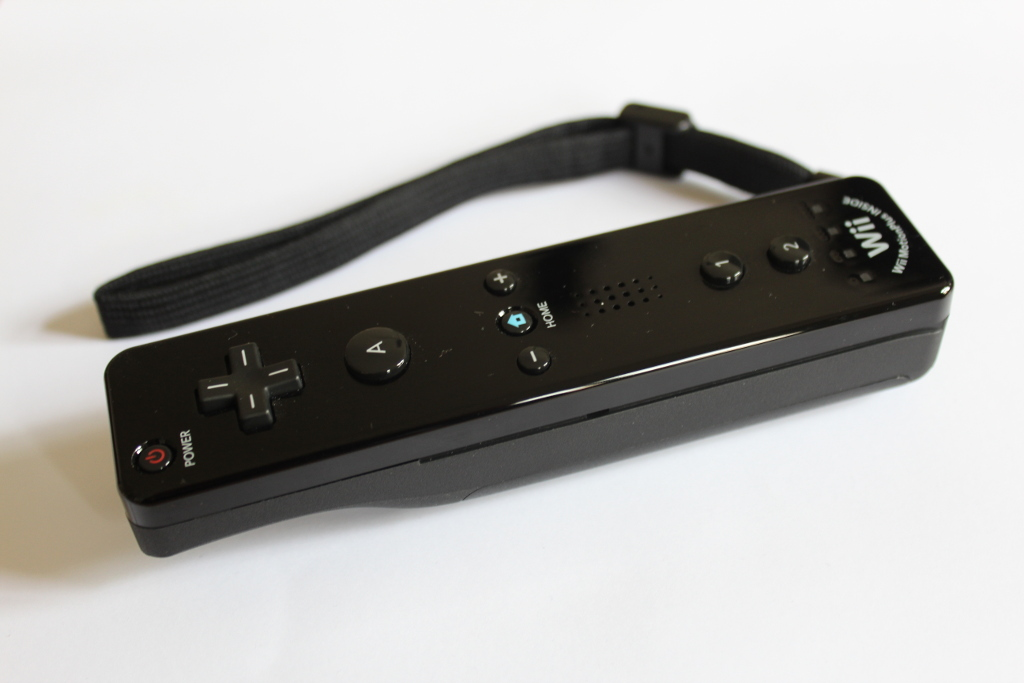
\includegraphics[width=0.5\textwidth]{wii-remote-plus-controller.JPG}
        \end{center}
    \end{itemize}
\end{frame}

\subsection{Data Recording Instructions} \label{data_recording_instructions}
The recording instructions of the experiment are containing 16 slides plus one slide for the welcoming and two slides
for thanking the experimentee and saying goodbye. The slides change after every performed gesture. A gesture can
be performed by pressing the \textit{B} button, moving the controller and releasing the \textit{B} button after the
gesture. As mentioned in section \ref{experiment}, the experiment consists of two parts, the recording of 8 training
gestures and the repetition of those gestures mixed with physical activities. All slides of the experiment are shown in
figure~\ref{fig:slides}.

\begin{figure}
    \begin{center}
        \resizebox {\textwidth} {!} {
            \begin{tabular}{cccc}
                \frame{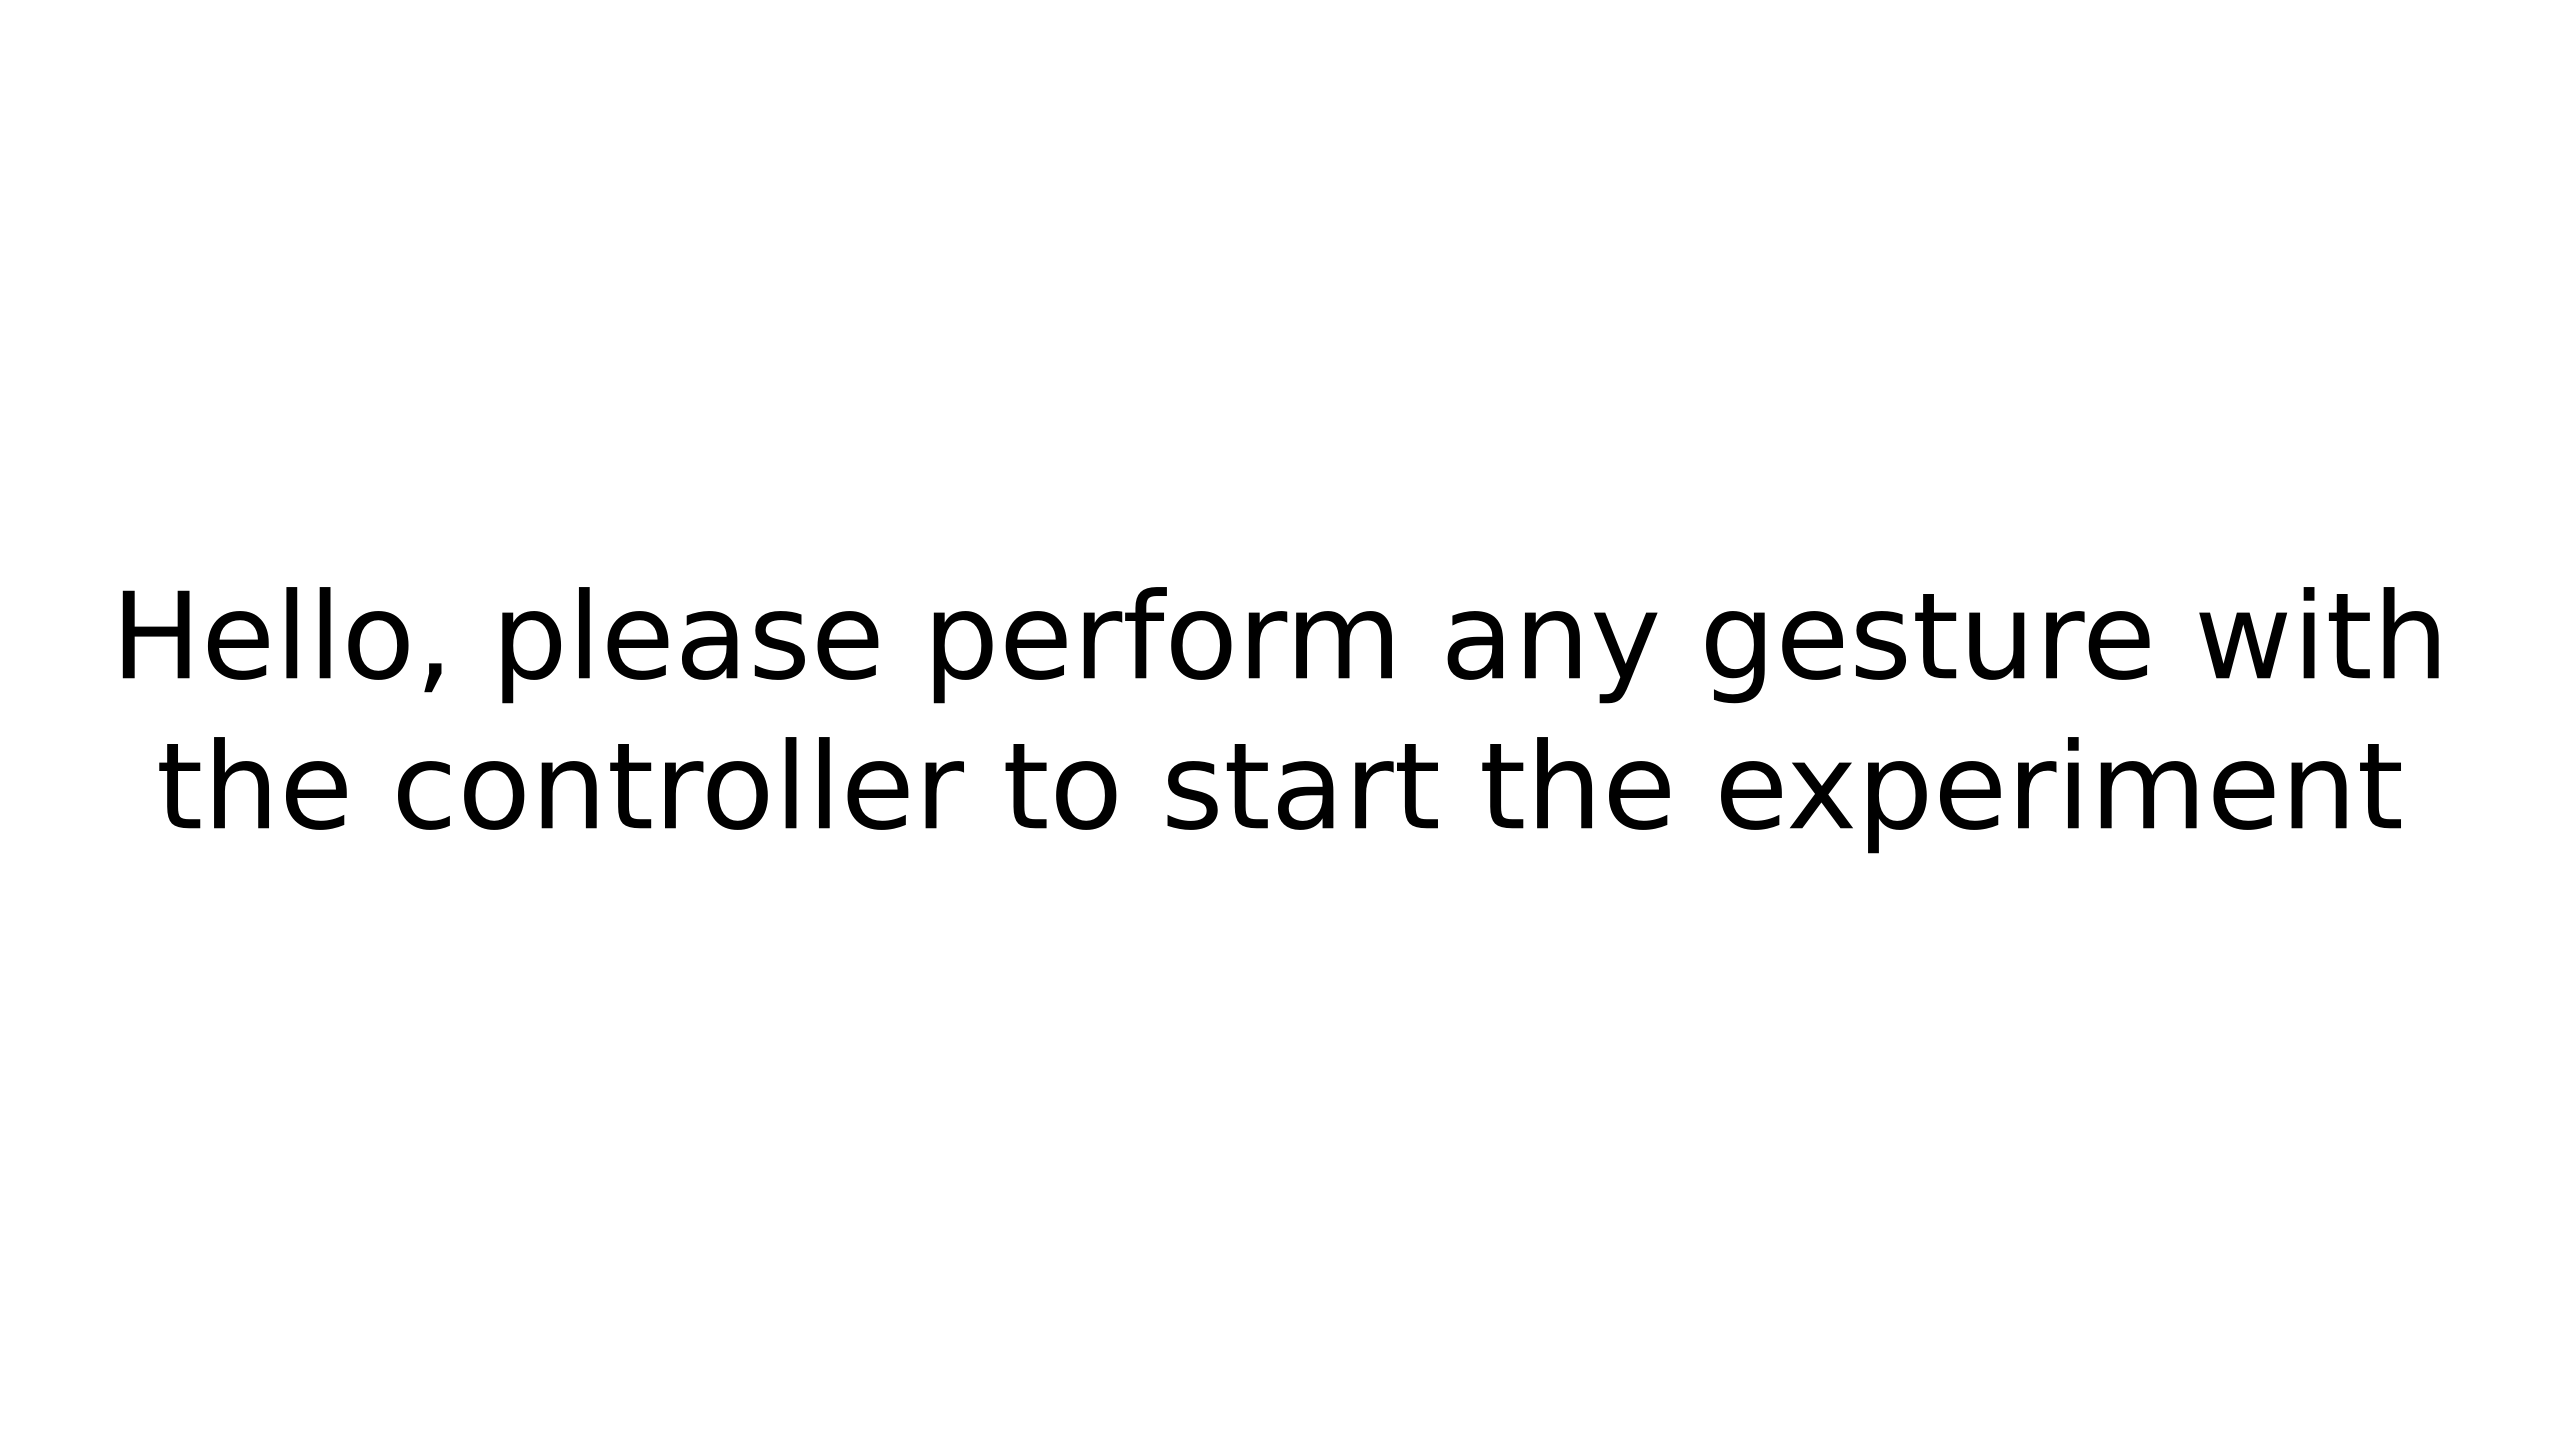
\includegraphics[width=0.25\textwidth]{1.png}} &
                \frame{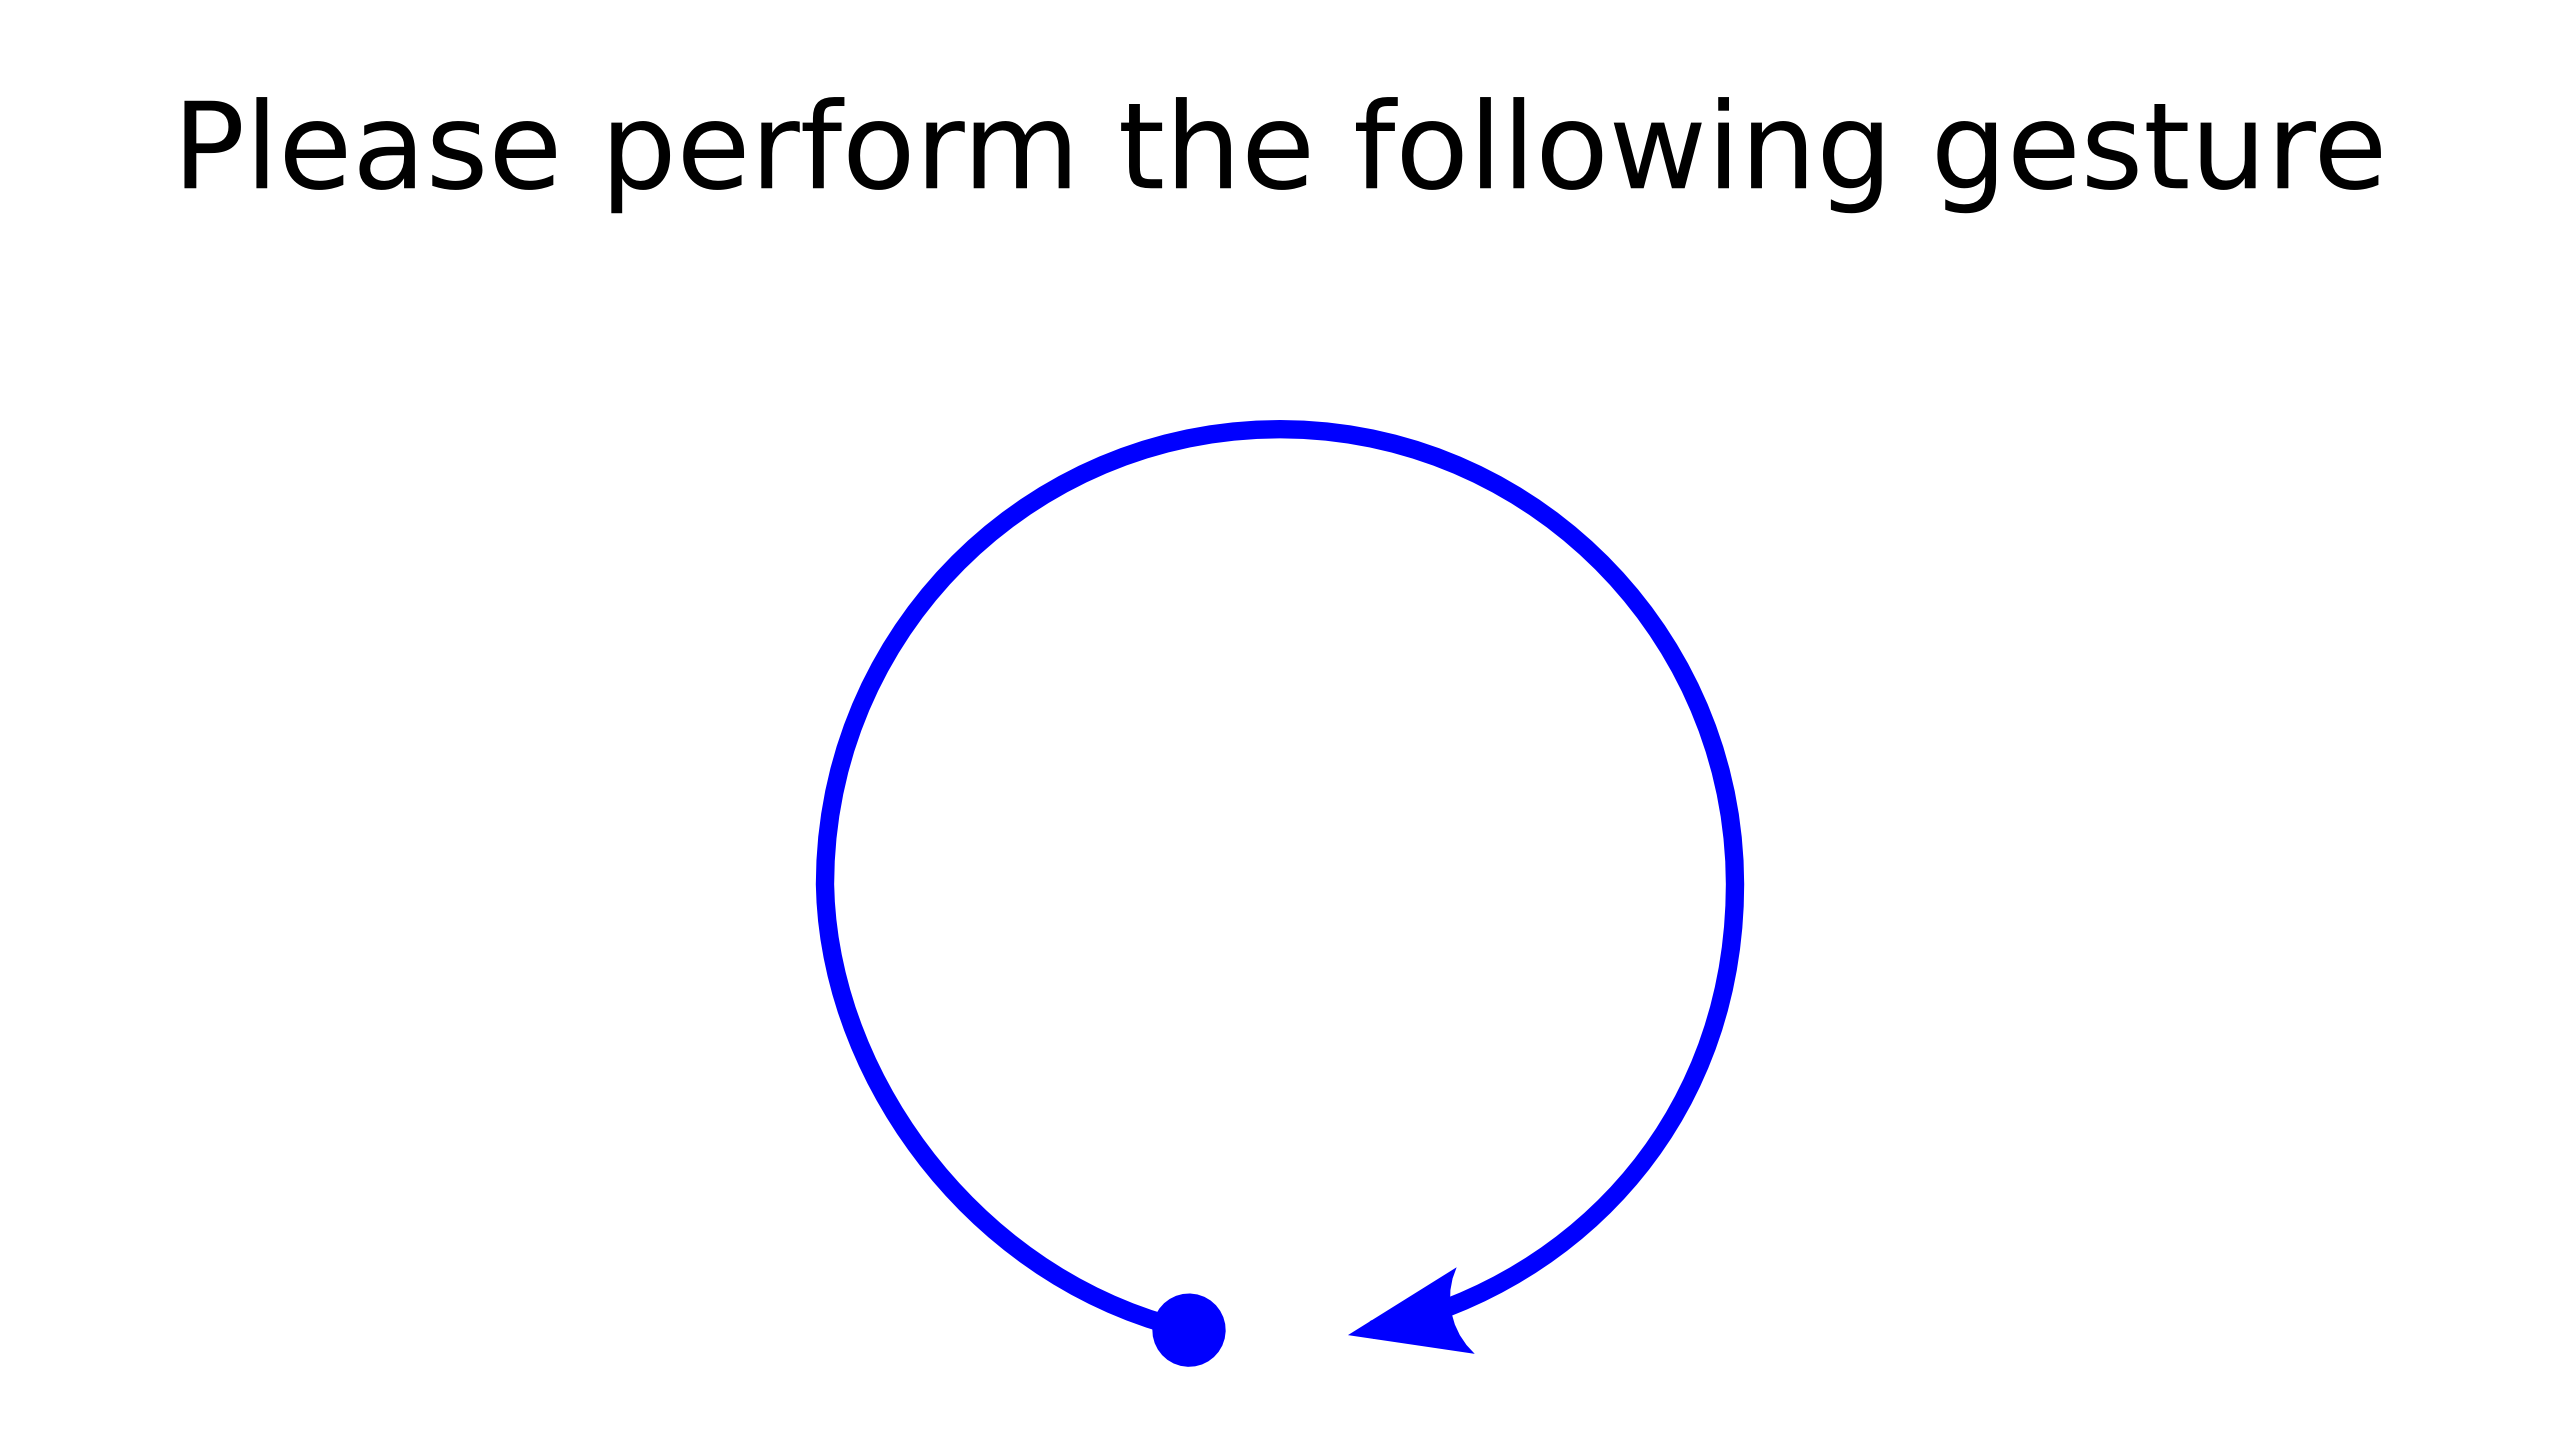
\includegraphics[width=0.25\textwidth]{2.png}} &
                \frame{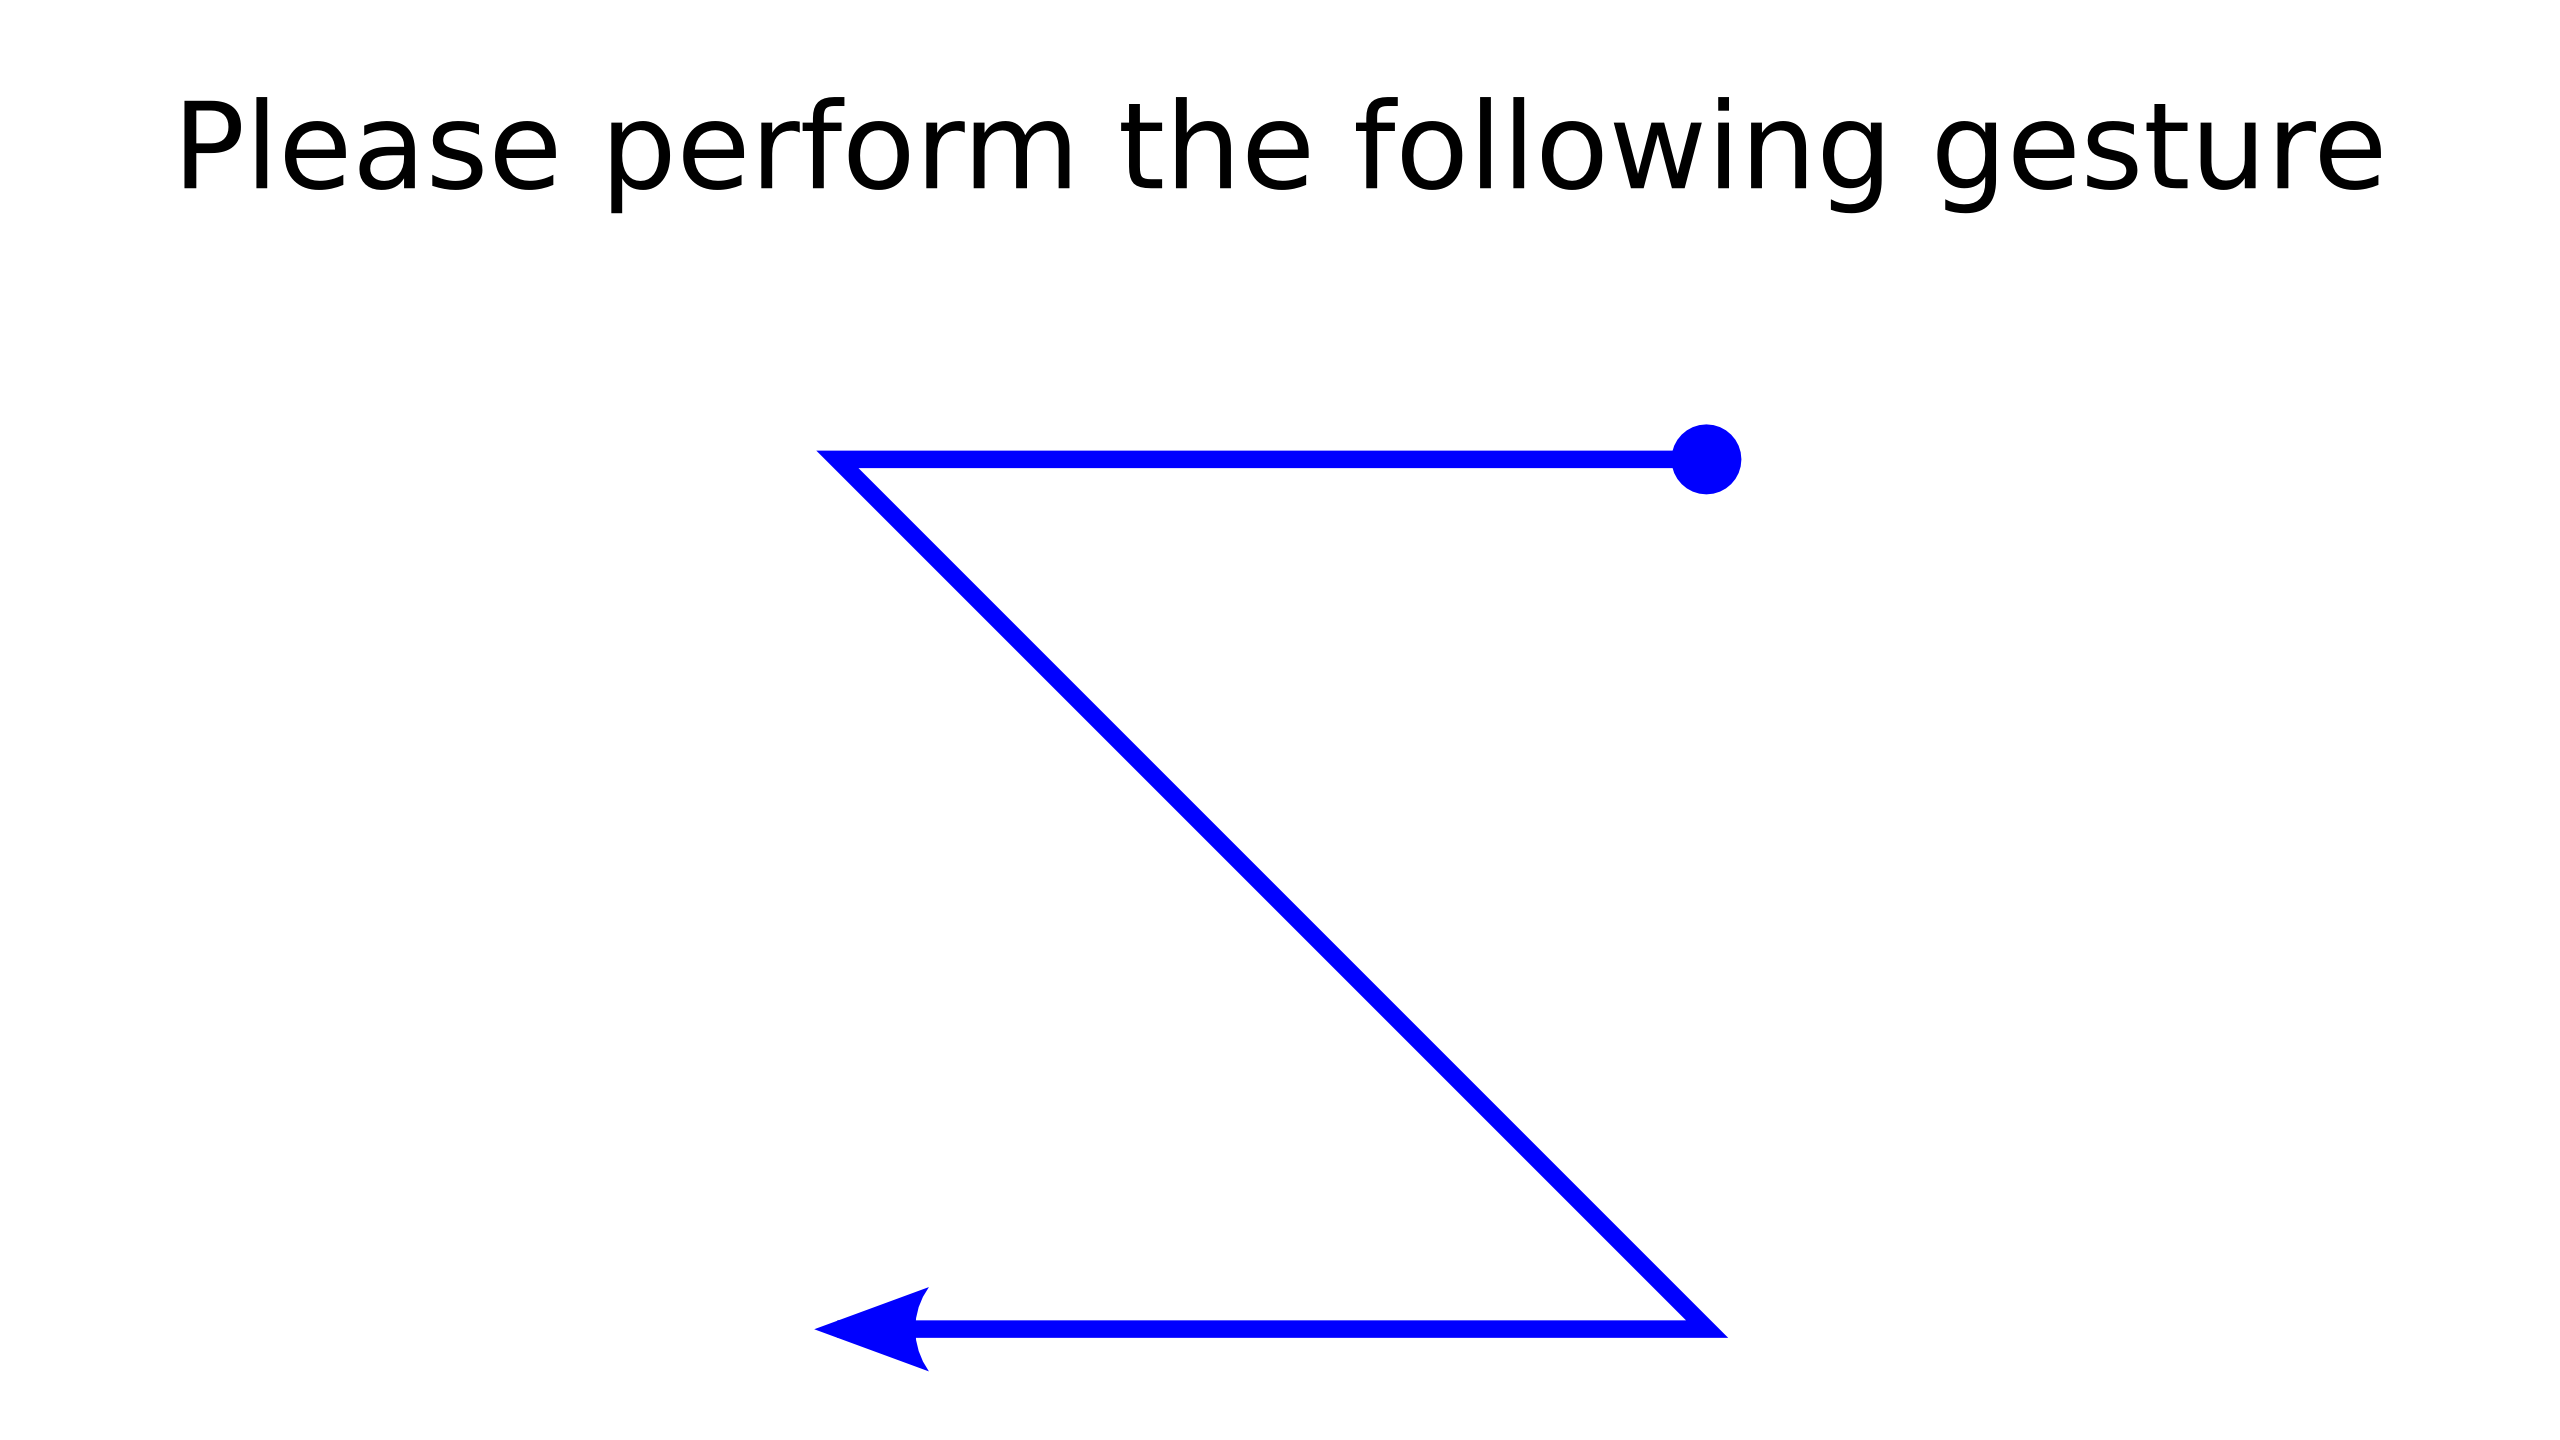
\includegraphics[width=0.25\textwidth]{3.png}} &
                \frame{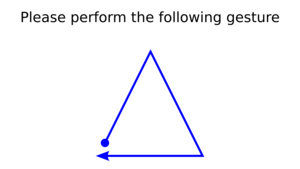
\includegraphics[width=0.25\textwidth]{4.png}} \\
                (a) \vspace{0.5ex} & (b) \vspace{0.5ex} & (c) \vspace{0.5ex} & (d) \vspace{0.5ex} \\
                \frame{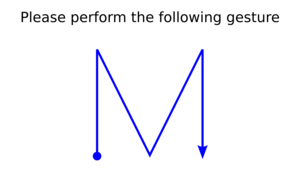
\includegraphics[width=0.25\textwidth]{5.png}} &
                \frame{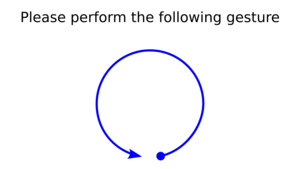
\includegraphics[width=0.25\textwidth]{6.png}} &
                \frame{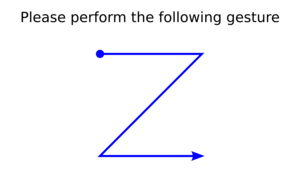
\includegraphics[width=0.25\textwidth]{7.png}} &
                \frame{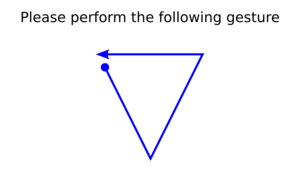
\includegraphics[width=0.25\textwidth]{8.png}} \\
                (e) \vspace{0.5ex} & (f) \vspace{0.5ex} & (g) \vspace{0.5ex} & (h) \vspace{0.5ex} \\
                \frame{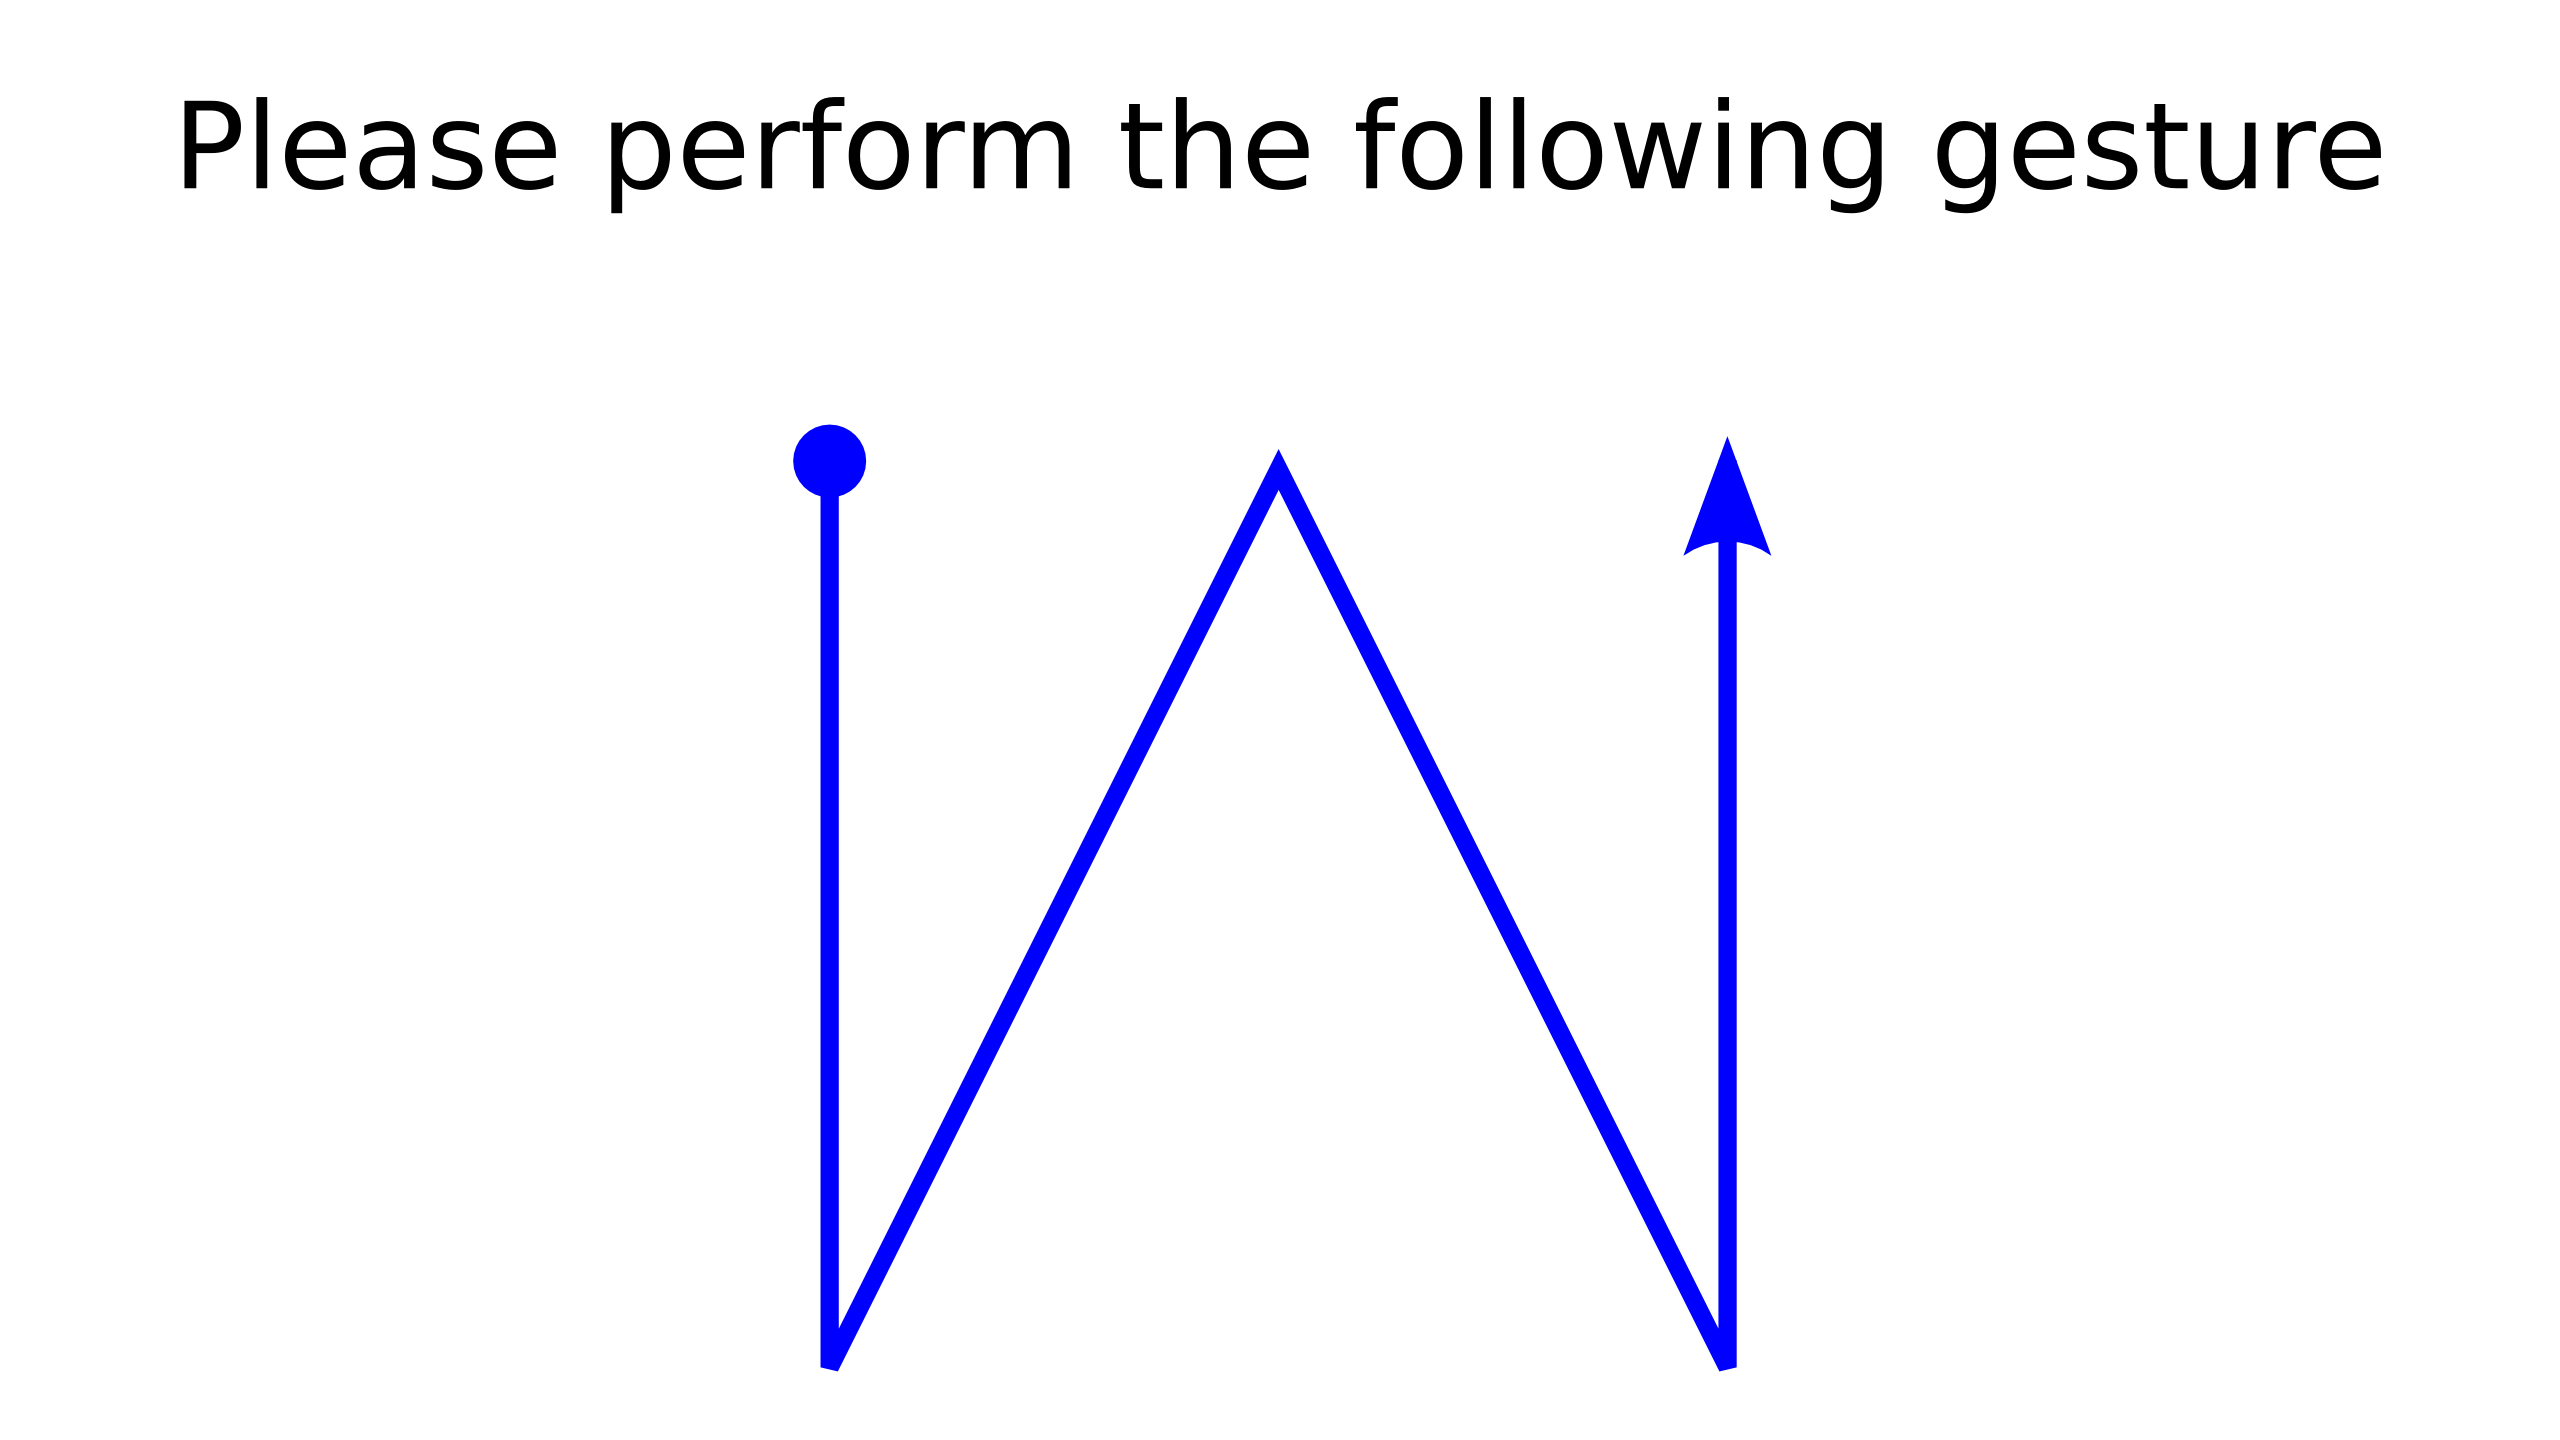
\includegraphics[width=0.25\textwidth]{9.png}} &
                \frame{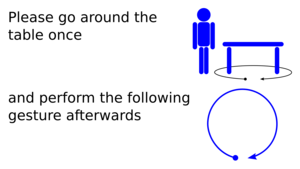
\includegraphics[width=0.25\textwidth]{10.png}} &
                \frame{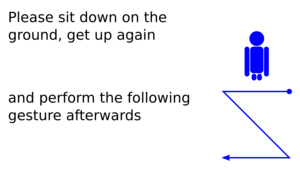
\includegraphics[width=0.25\textwidth]{11.png}} &
                \frame{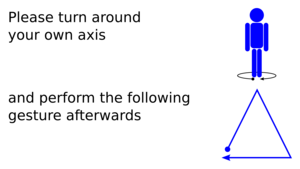
\includegraphics[width=0.25\textwidth]{12.png}} \\
                (i) \vspace{0.5ex} & (j) \vspace{0.5ex} & (k) \vspace{0.5ex} & (l) \vspace{0.5ex} \\
                \frame{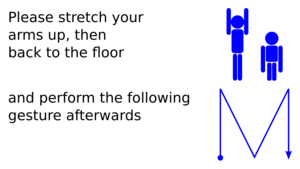
\includegraphics[width=0.25\textwidth]{13.png}} &
                \frame{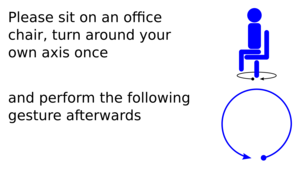
\includegraphics[width=0.25\textwidth]{14.png}} &
                \frame{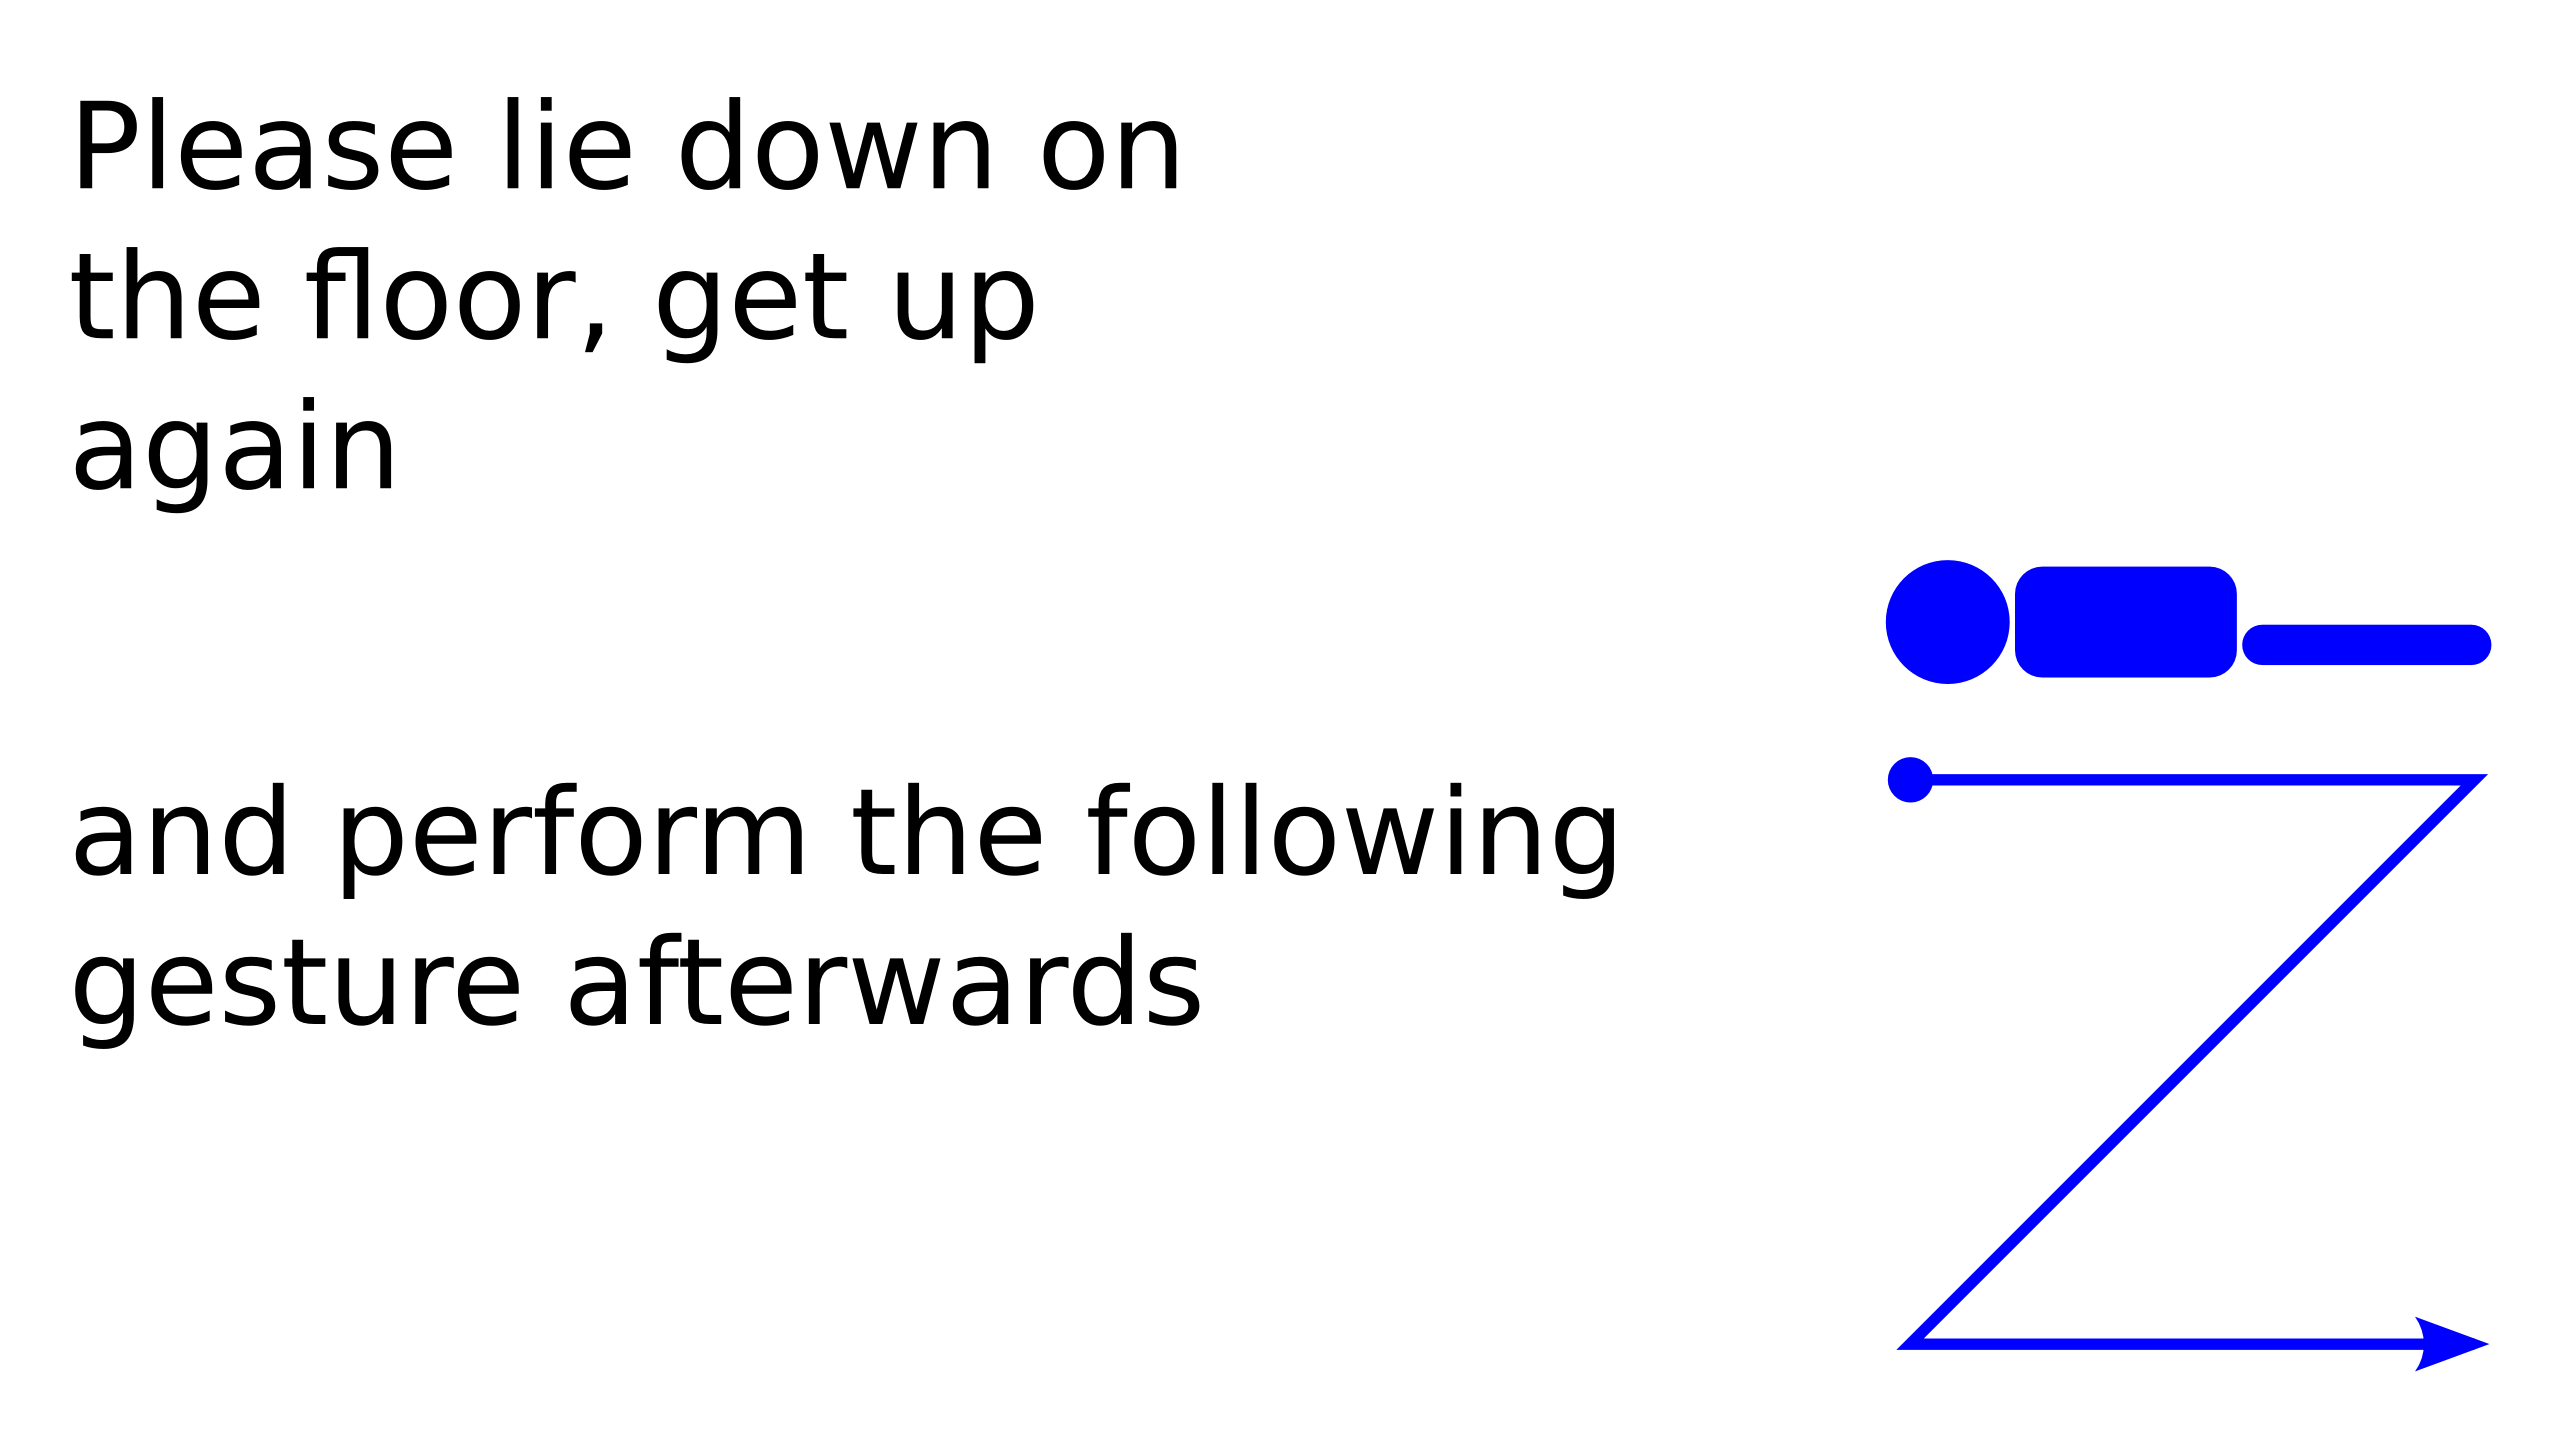
\includegraphics[width=0.25\textwidth]{15.png}} &
                \frame{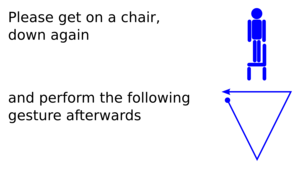
\includegraphics[width=0.25\textwidth]{16.png}} \\
                (m) \vspace{0.5ex} & (n) \vspace{0.5ex} & (o) \vspace{0.5ex} & (p) \vspace{0.5ex} \\
                \frame{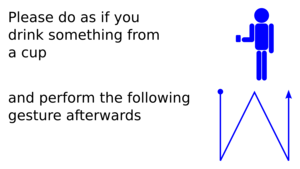
\includegraphics[width=0.25\textwidth]{17.png}} &
                \frame{
\includegraphics[width=0.25\textwidth]{18.png}} &
                \frame{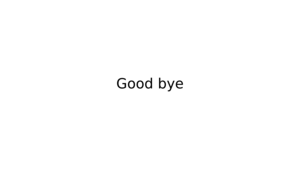
\includegraphics[width=0.25\textwidth]{19.png}} & \\
                (q) & (r) & (s) & \\
            \end{tabular}
        }
    \end{center}
    \caption{The slides that are guiding the experimentees.}
    \label{fig:slides}
\end{figure}

Slide (a) of figure \ref{fig:slides} has the task to welcome the experimentee and is later used in experimental protocol
to mark the start of the recording. The slides (b) to (i) of figure \ref{fig:slides} have the task to create training
data for 1NN-DTW. Physical activities mixed with the same gestures from (b) to (i) are on the slides (j) to (q) of
figure \ref{fig:slides}. The recorded acceleration data from slide (j) to (q) of figure \ref{fig:slides} will simulate
the time series stream in section \ref{experimental_protocol}. Slide (r) of figure \ref{fig:slides} and the last
insignificant gesture have the task to prevent an abrupt ending of the record. The last slide (s) of figure
\ref{fig:slides} closes the recording applciation.

\subsubsection{Gesture Notation} \label{gesture_notation}
The \textit{clockwise circle} gesture of slide (b) and (j) in figure \ref{fig:slides} is abbreviated with $GesA$, the
\textit{flipped Z} gesture on slide (c) and (k) of figure \ref{fig:slides} is abbreviated with $GesB$ and so on until
the \textit{W} gesture of slide (i) and (q) in figure \ref{fig:slides} shortend with $GesH$.

As the experiment was executed by different experimentees a instance of gesture $GesC$ performed by the fourth
experimentee on slide (d) of figure \ref{fig:slides} will be abbreviated as $exp_{4}.GesC_{1}$. The same gesture by the
same experimentee on slide (l) of figure \ref{fig:slides} will be abbreviated as $exp_{4}.GesC_{2}$.


\subsection{Experimental Protocol} \label{experimental_protocol}
The software to evaluate the recorded data has been written in Java\footnote{https://www.java.com/} and is available on
GitHub\footnote{https://github.com/GordonLesti/SlidingWindowFilter-evaluator}. The requirements are
OpenJDK\footnote{http://openjdk.java.net/} 8 to run the code and Gradle\footnote{https://gradle.org/} 3.3 to test the
code and build the executable binaries.

\subsubsection{Quantization} \label{quantization}
All recorded data were quantized before evaluation. The authors of \cite{liu2009uwave} have two reasons for that,
the length of the time series were reduced for DTW in order to improve computation efficiency and the recorded time
series was transformed with a stable time gab between the data points. The quantization process of
\cite{liu2009uwave} is used in this bachelor thesis. The quantization process of a recorded gesture is
illustrated by figure \ref{fig:quantization}.

\paragraph{Compressing} The recorded acceleration data were compressed to an average value for a window size of 50
ms and a step length of 30 ms.

\paragraph{Conversion} The compressed records are converted into 33 different levels that are summarized in
table \ref{table:conversion}.

\begin{table}
    \begin{center}
        \begin{tabularx}{\textwidth}{XX}
            \hline
            \textbf{Acceleration data ($a$) in $\frac{dm}{s^2}$} & \qquad \textbf{Converted value}\\
            \hline
            $a > 200$ & \qquad 16\\
            $100 < a < 200$ & \qquad 11 to 15 (five levels linearly)\\
            $0 < a < 100$ & \qquad 1 to 10 (ten levels linearly)\\
            $a = 0$ & \qquad 0\\
            $-100 < a < 0$ & \qquad -1 to - 10 (ten levels linearly)\\
            $-200 < a < -100$ & \qquad -11 to - 15 (five levels linearly)\\
            $a < -200$ & \qquad -16\\
            \hline
        \end{tabularx}
    \end{center}
    \caption{Table shows the conversion rules of the recorded acceleration data. In contrast to \cite{liu2009uwave} are
    $100\frac{dm}{s^2}$ the steps threshold and not $1g$.}
	\label{table:conversion}
\end{table}

\begin{figure}
    \begin{center}
        \resizebox {\textwidth} {!} {
            \begin{tabular}{ccc}
                \resizebox {!} {\height} {
                    \begin{tikzpicture}
                        \begin{axis}[
                            xmin=1,
                            xmax=295,
                            xlabel=time,
                            ylabel=acceleration in $\frac{dm}{s^2}$]
                            \addplot[blue, ultra thick, mark=none] table[x=t, y=x] {experiment/experimental_protocol/quantization/raw.dat};
                            \addplot[red, ultra thick, mark=none] table[x=t, y=y] {experiment/experimental_protocol/quantization/raw.dat};
                            \addplot[green, ultra thick, mark=none] table[x=t, y=z] {experiment/experimental_protocol/quantization/raw.dat};
                        \end{axis}
                    \end{tikzpicture}
                } &
                \resizebox {!} {\height} {
                    \begin{tikzpicture}
                        \pgfplotsset{every axis legend/.append style={
                    		at={(0.5,1.03)},
                    		anchor=south}}
                        \begin{axis}[
                            xmin=1,
                            xmax=52,
                            xlabel=time,
                            ylabel=acceleration in $\frac{dm}{s^2}$,
                            legend columns=4]
                            \addplot[blue, ultra thick, mark=none] table[x=t, y=x] {experiment/experimental_protocol/quantization/compressed.dat};
                            \addlegendentry{x-axis}
                            \addplot[red, ultra thick, mark=none] table[x=t, y=y] {experiment/experimental_protocol/quantization/compressed.dat};
                            \addlegendentry{y-axis}
                            \addplot[green, ultra thick, mark=none] table[x=t, y=z] {experiment/experimental_protocol/quantization/compressed.dat};
                            \addlegendentry{z-axis}
                        \end{axis}
                    \end{tikzpicture}
                } &
                \resizebox {!} {\height} {
                    \begin{tikzpicture}
                        \begin{axis}[
                            xmin=1,
                            xmax=52,
                            xlabel=time,
                            ylabel=converted acceleration]
                            \addplot[blue, ultra thick, mark=none] table[x=t, y=x] {experiment/experimental_protocol/quantization/converted.dat};
                            \addplot[red, ultra thick, mark=none] table[x=t, y=y] {experiment/experimental_protocol/quantization/converted.dat};
                            \addplot[green, ultra thick, mark=none] table[x=t, y=z] {experiment/experimental_protocol/quantization/converted.dat};
                        \end{axis}
                    \end{tikzpicture}
                }
            \end{tabular}
        }
    \end{center}
    \caption{The left plot shows the raw recorded gesture for all three axis. On the middle plot are the compressed
    acceleration data of the gesture. The right plot shows the converted and compressed gesture.}
    \label{fig:quantization}
\end{figure}

\subsubsection{Labeled Generic Time Series Model} \label{labeled_generic_time_series_model}
A generic time series model was created for the evaluating software. A generic time series over the domain set
$\mathbb{U}$ will be a linked list of data points. Those data points are containing a generic data object and an
optional label. The generic object has to be an element of the domain set $\mathbb{U}$. In the case of the carried out
experiment a data point contains the acceleration data of the x-axis, the y-axis and z-axis. So $\mathbb{U}$ will be
similar to $\mathbb{Z}^3$. $\mathbb{U}$ will be the set of vectors containing three integer values and the distance
function $D$ on $\mathbb{U}$ will be the eucliean distance $\sqrt[2]{(x_1 - x_2)^2 + (y_1 - y_2)^2 + (z_1 - z_2)^2}$.
The generic approach for the implemented time series model and the time series measures should make it easier to
evaluate similar experiments on other domains. A label of a data point will be used to mark a data point as part of a
gesture.

\subsubsection{Sliding Window Simulation} \label{sliding_window_simulation}
A sliding window simulation walks with a given window size and step size over the simulated acceleration time series
stream of an experimentee and tries to identify as many gestures as possible. The simulated acceleration time series
stream of an experimentee starts after the slide (j) of figure \ref{fig:slides} and ends in slide (r) of figure
\ref{fig:slides}. The sliding window simulation is not able to read the labels of an gesture in the simulated
acceleration time series. Furthermore a sliding window simulation gets the gestures of an experimentee from slide (b)
to (i) in figure \ref{fig:slides} as training data.

Such a simulation is not free of parameters. Two parameters are already mentioned, the window size and the steps
size. In addition to parameters being the choice of the distance measure for time series, the threshold that marks
unclassifiable windows and the measure used for the sliding window filter with a blur factor. All those parameters and
their options are explained and mentioned in the following section. Furthermore a performance measure to compare the
different configured simulations is explained.

\input{experiment/experimental_protocol/sliding_window_simulation/window_size_determination.tex}
\input{experiment/experimental_protocol/sliding_window_simulation/step_size_determination.tex}
\input{experiment/experimental_protocol/sliding_window_simulation/time_series_distance_measures.tex}
\input{experiment/experimental_protocol/sliding_window_simulation/threshold_determination.tex}
\input{experiment/experimental_protocol/sliding_window_simulation/sliding_window_filter_measures.tex}
\input{experiment/experimental_protocol/sliding_window_simulation/performance_measure.tex}


\section{Evaluation}

\begin{frame}{Evaluation}
    \begin{itemize}
        \item Accelerometer-based gesture detection inspired by \textit{uWave} \cite{liu2009uwave}

        \item 14 records of three-dimensional acceleration time series by 14 different experimentees

        \item Recorded via a Wii Remote\texttrademark~Plus Wii U is a trademark of Nintendo. controller
        \begin{center}
            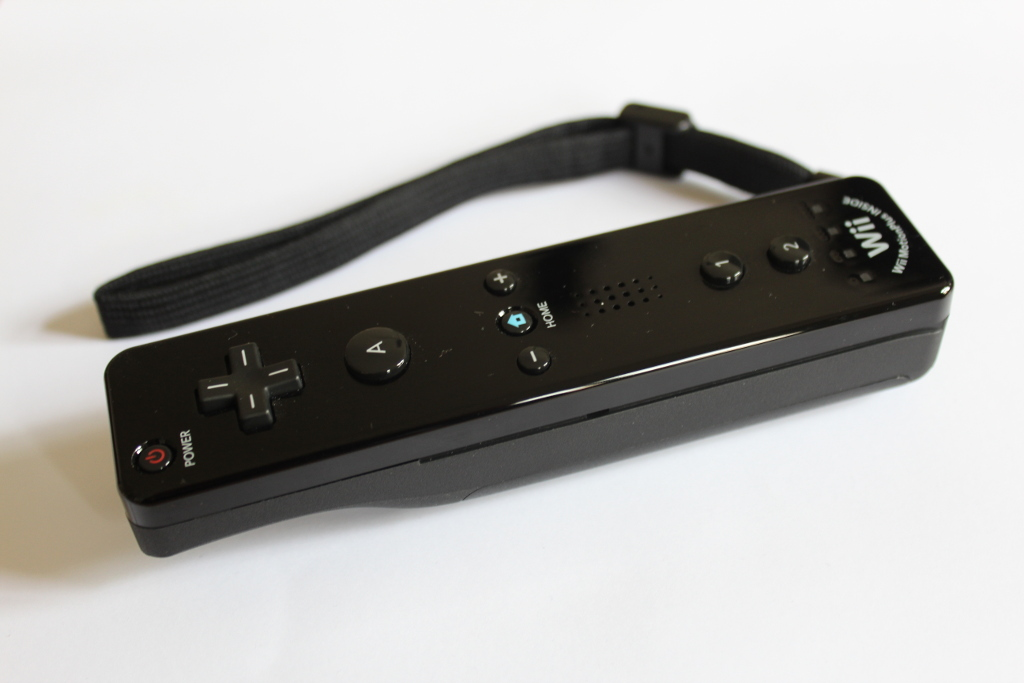
\includegraphics[width=0.5\textwidth]{wii-remote-plus-controller.JPG}
        \end{center}
    \end{itemize}
\end{frame}

\begin{frame}{Evaluation}{Data Recording Instructions}
    \begin{center}
        \resizebox {\textwidth} {!} {
            \begin{tabular}{ccccc}
                \frame{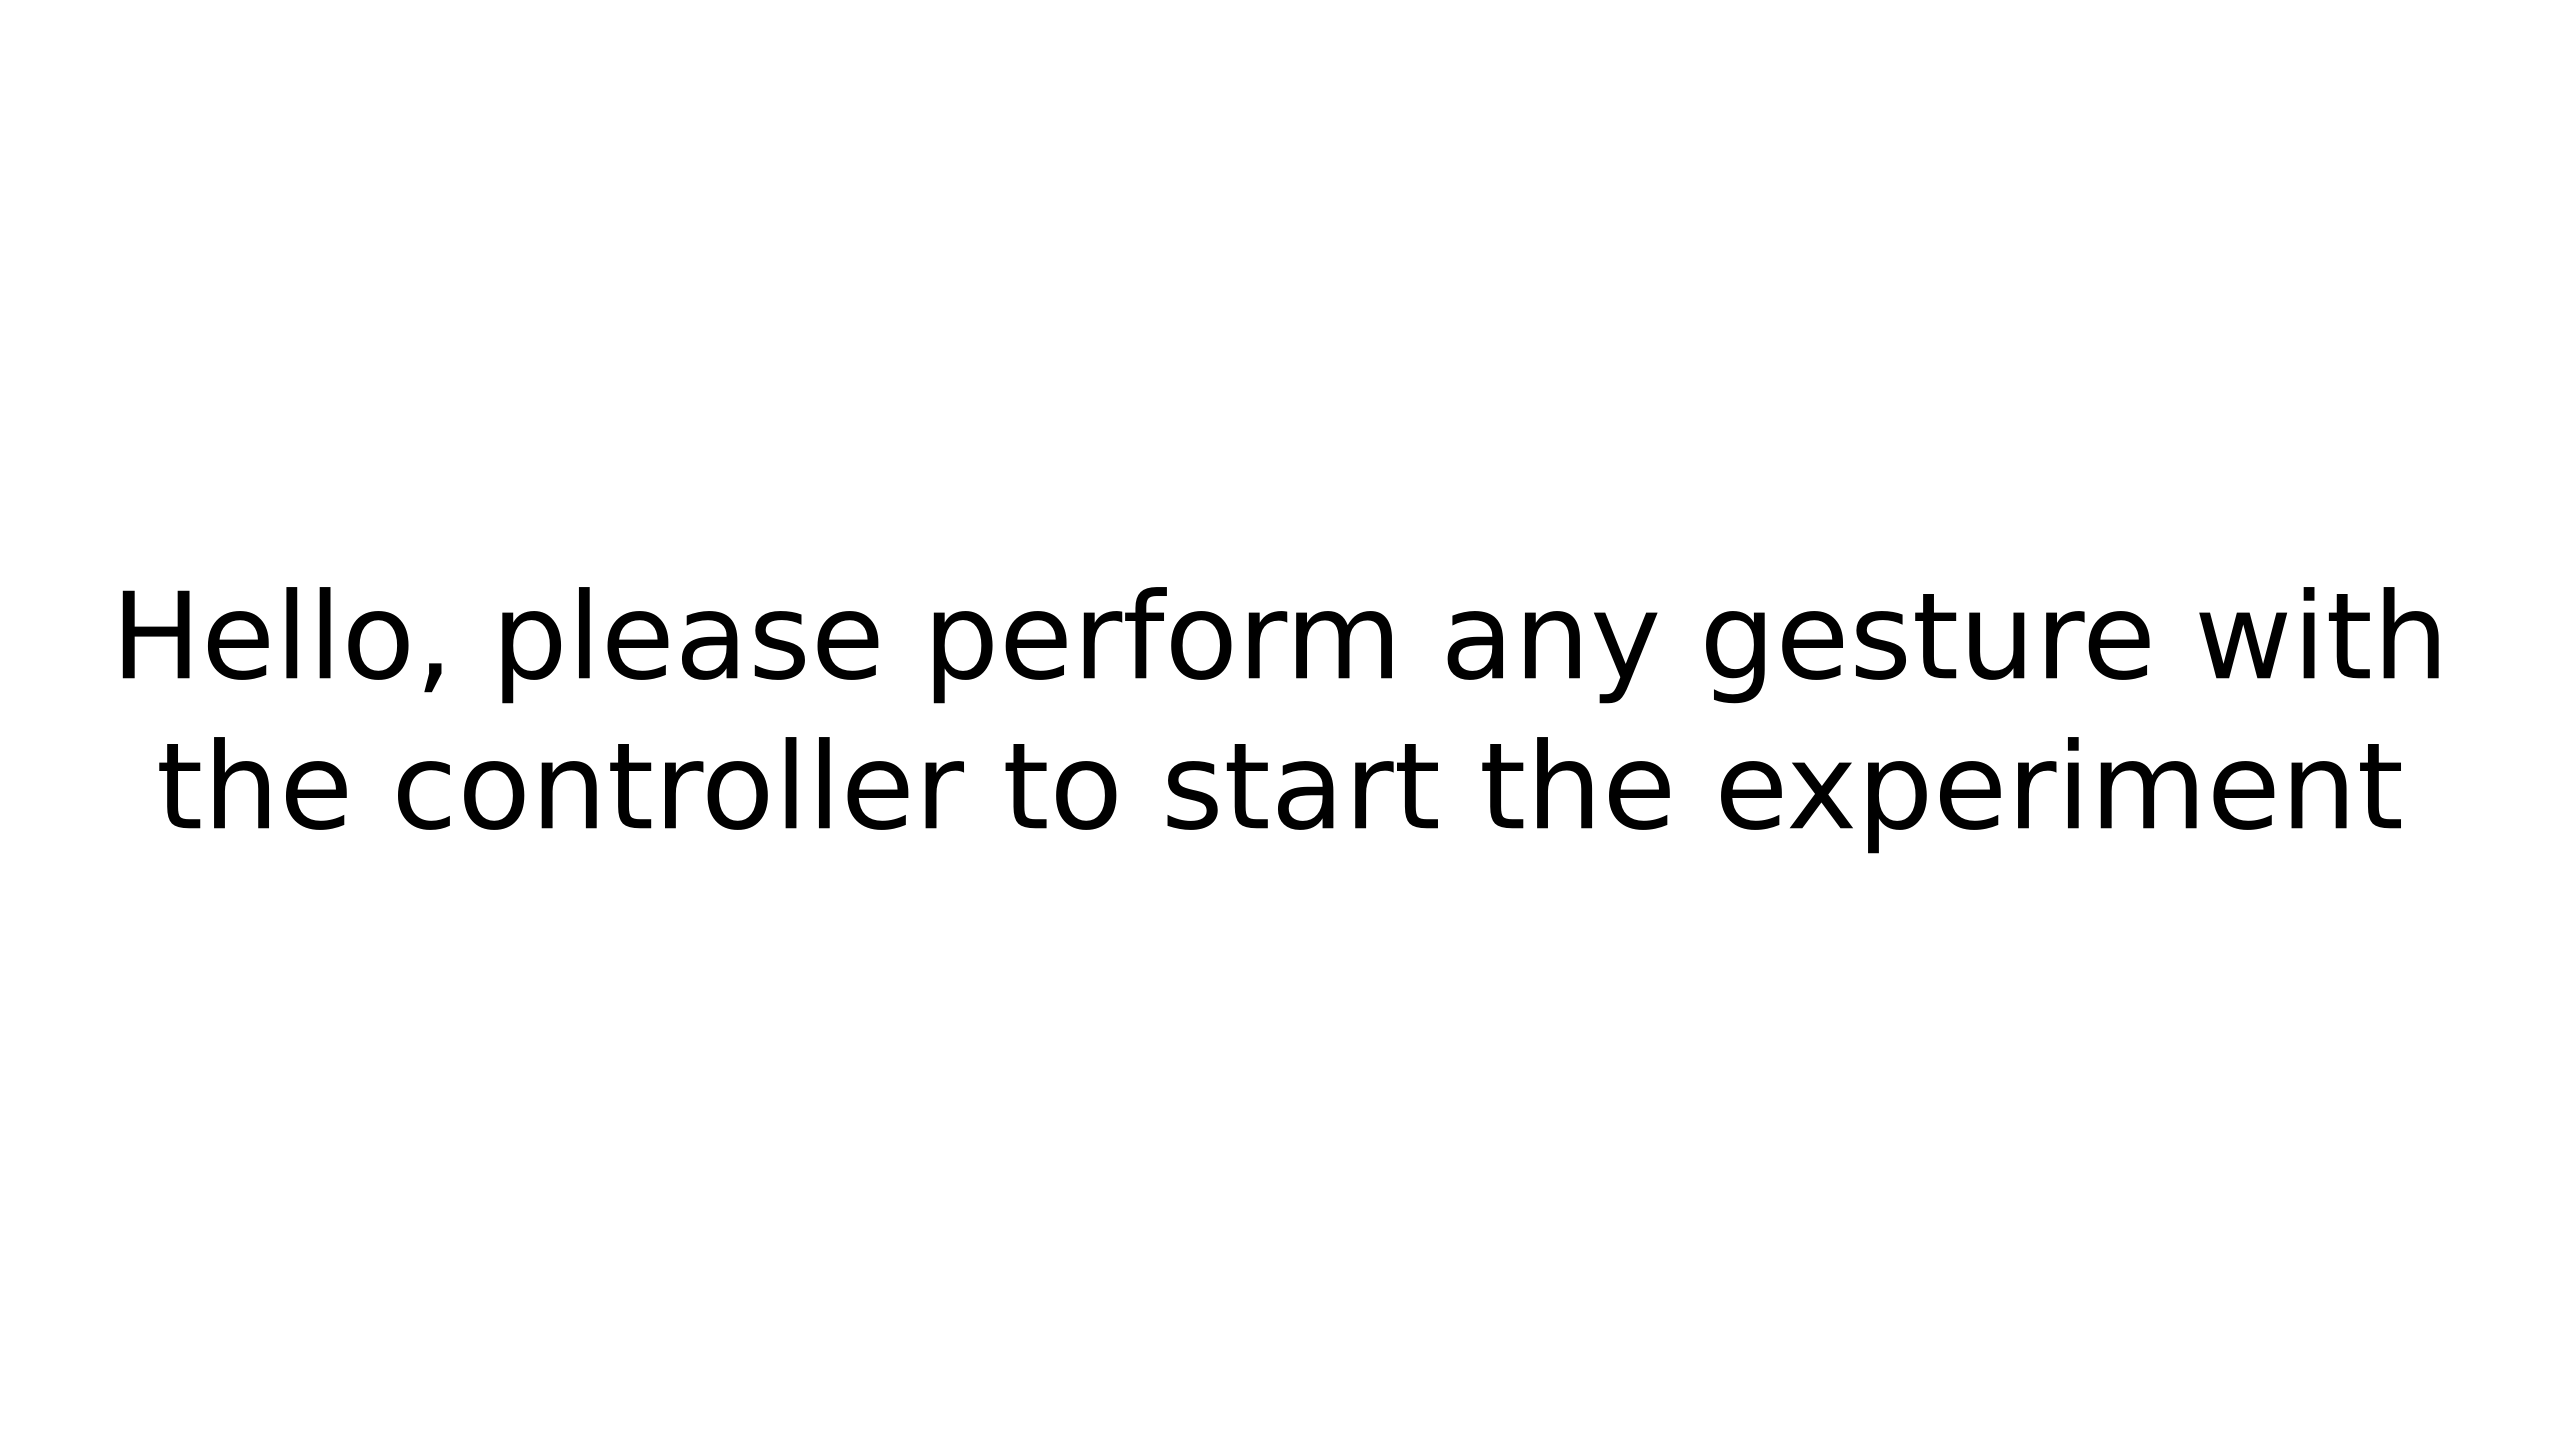
\includegraphics[width=0.25\textwidth]{1.png}} &
                \frame{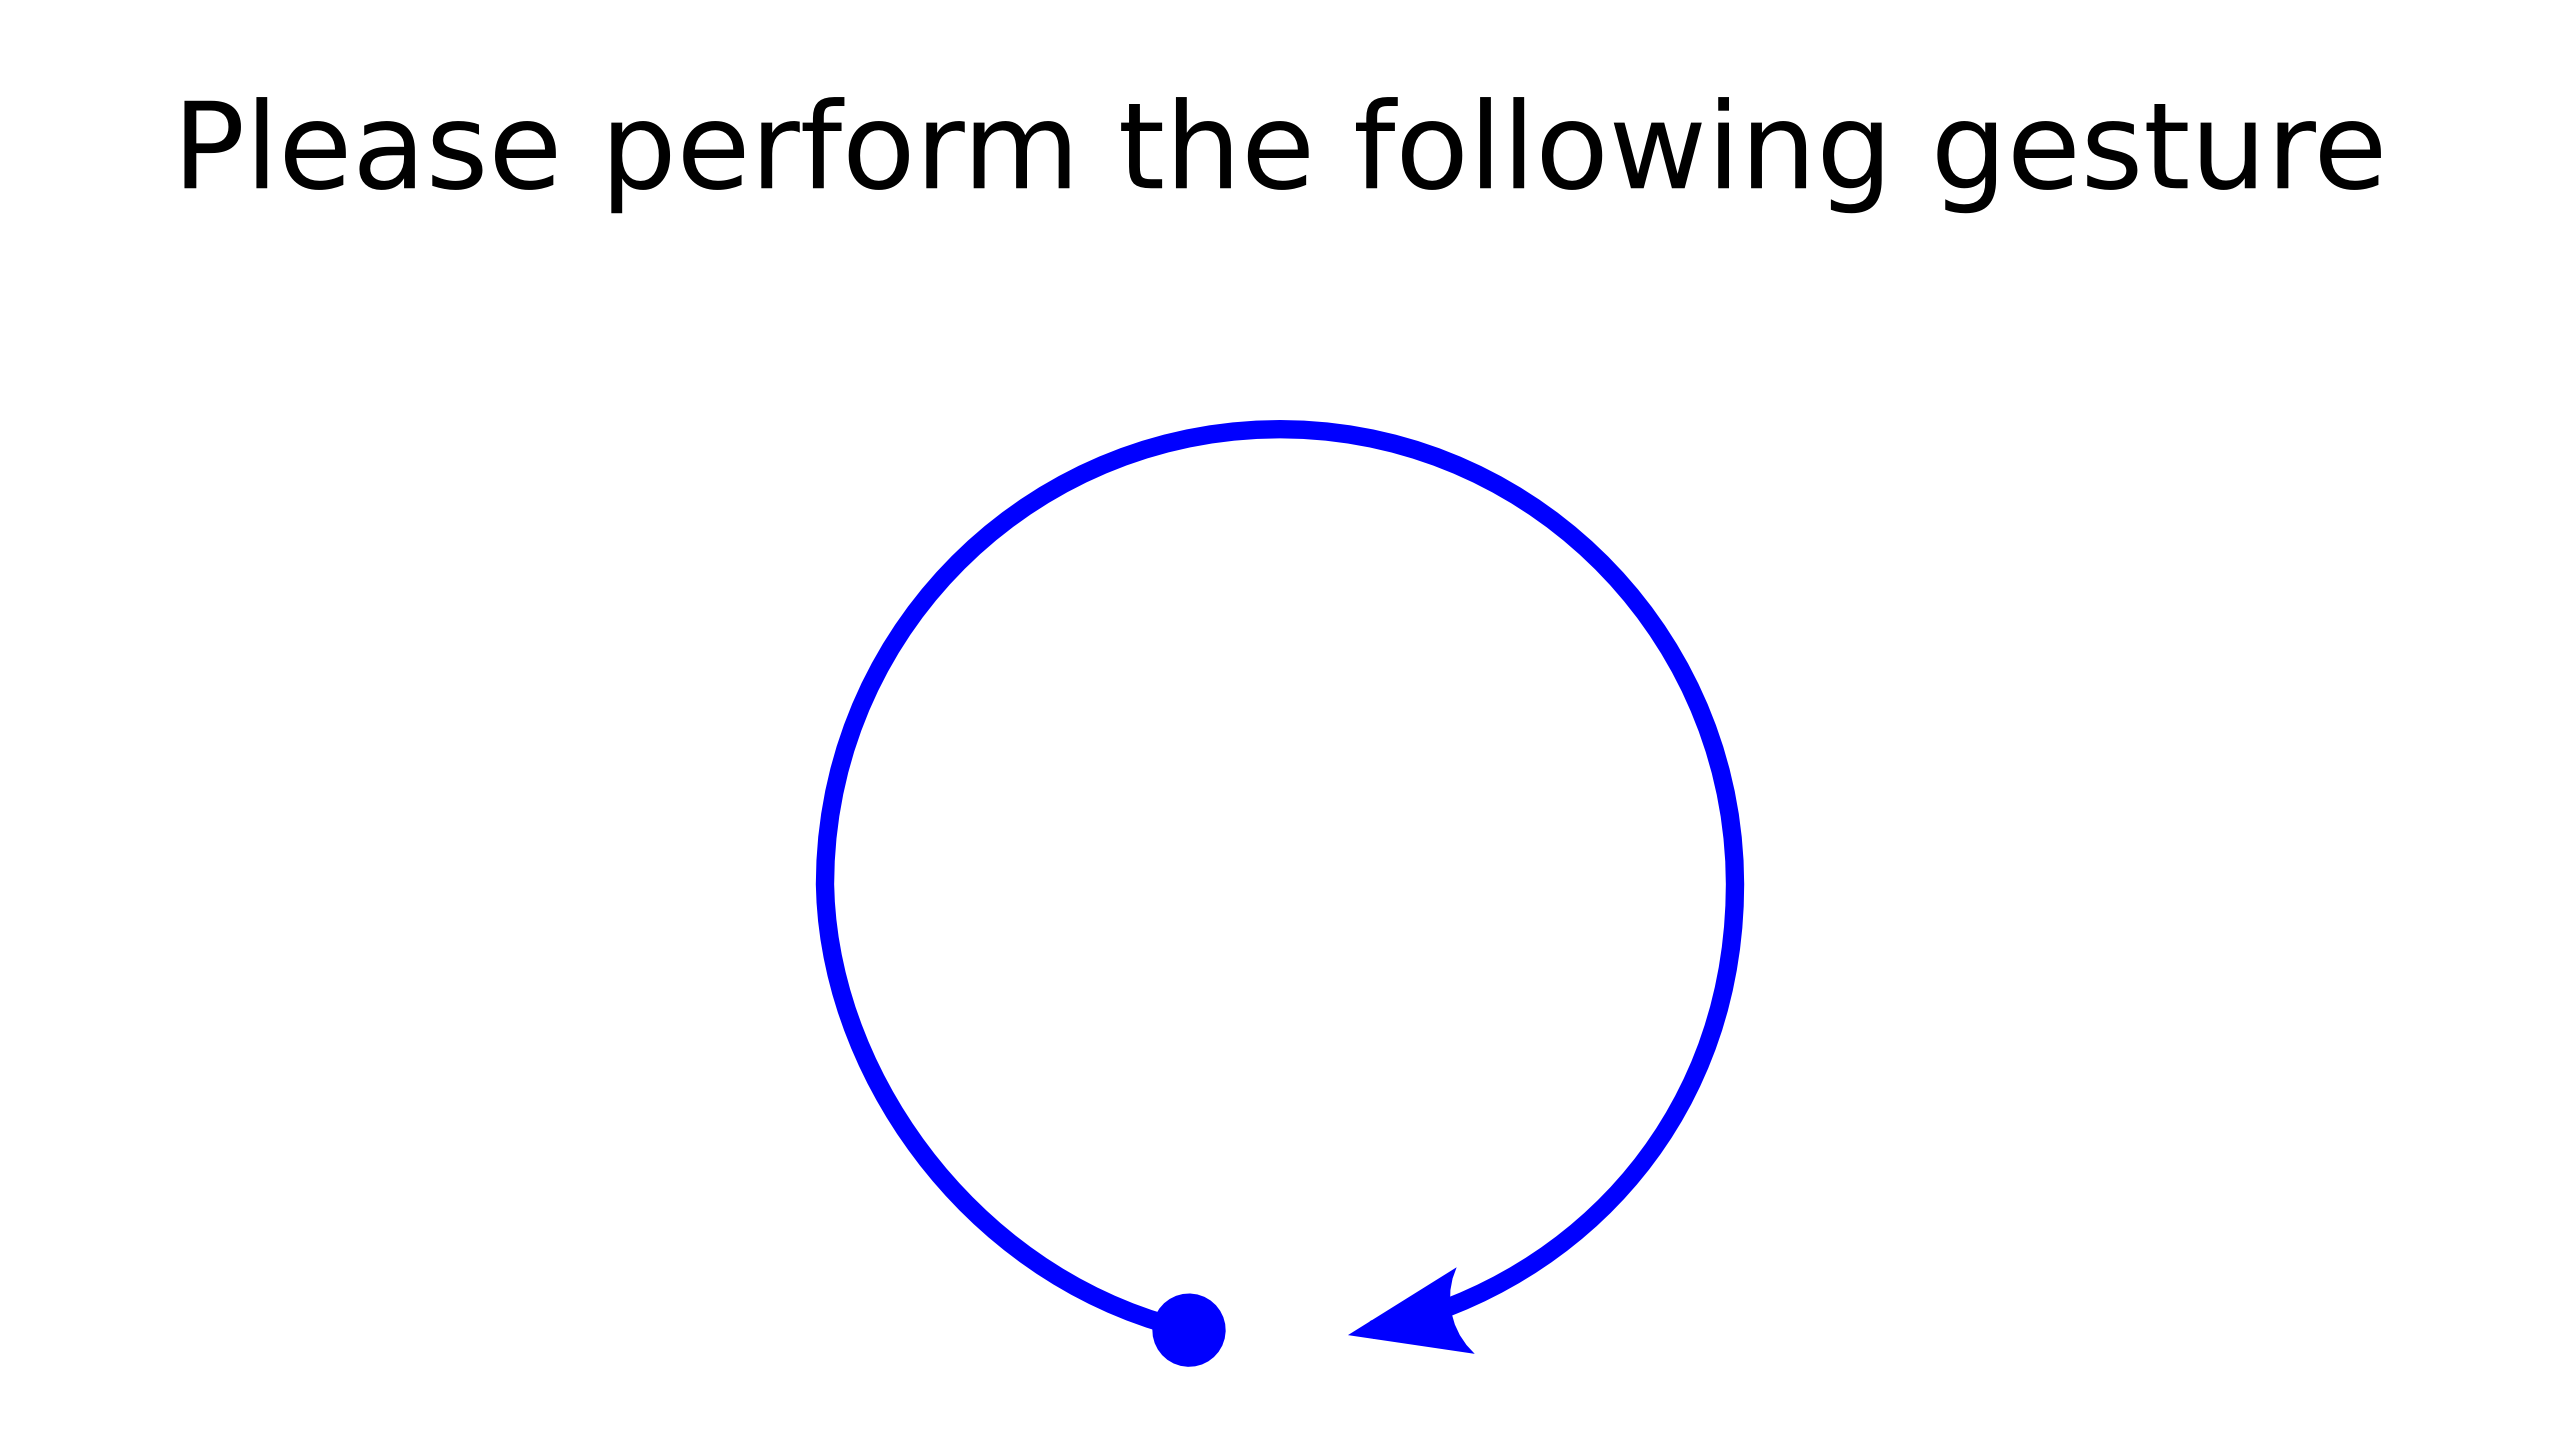
\includegraphics[width=0.25\textwidth]{2.png}} &
                \frame{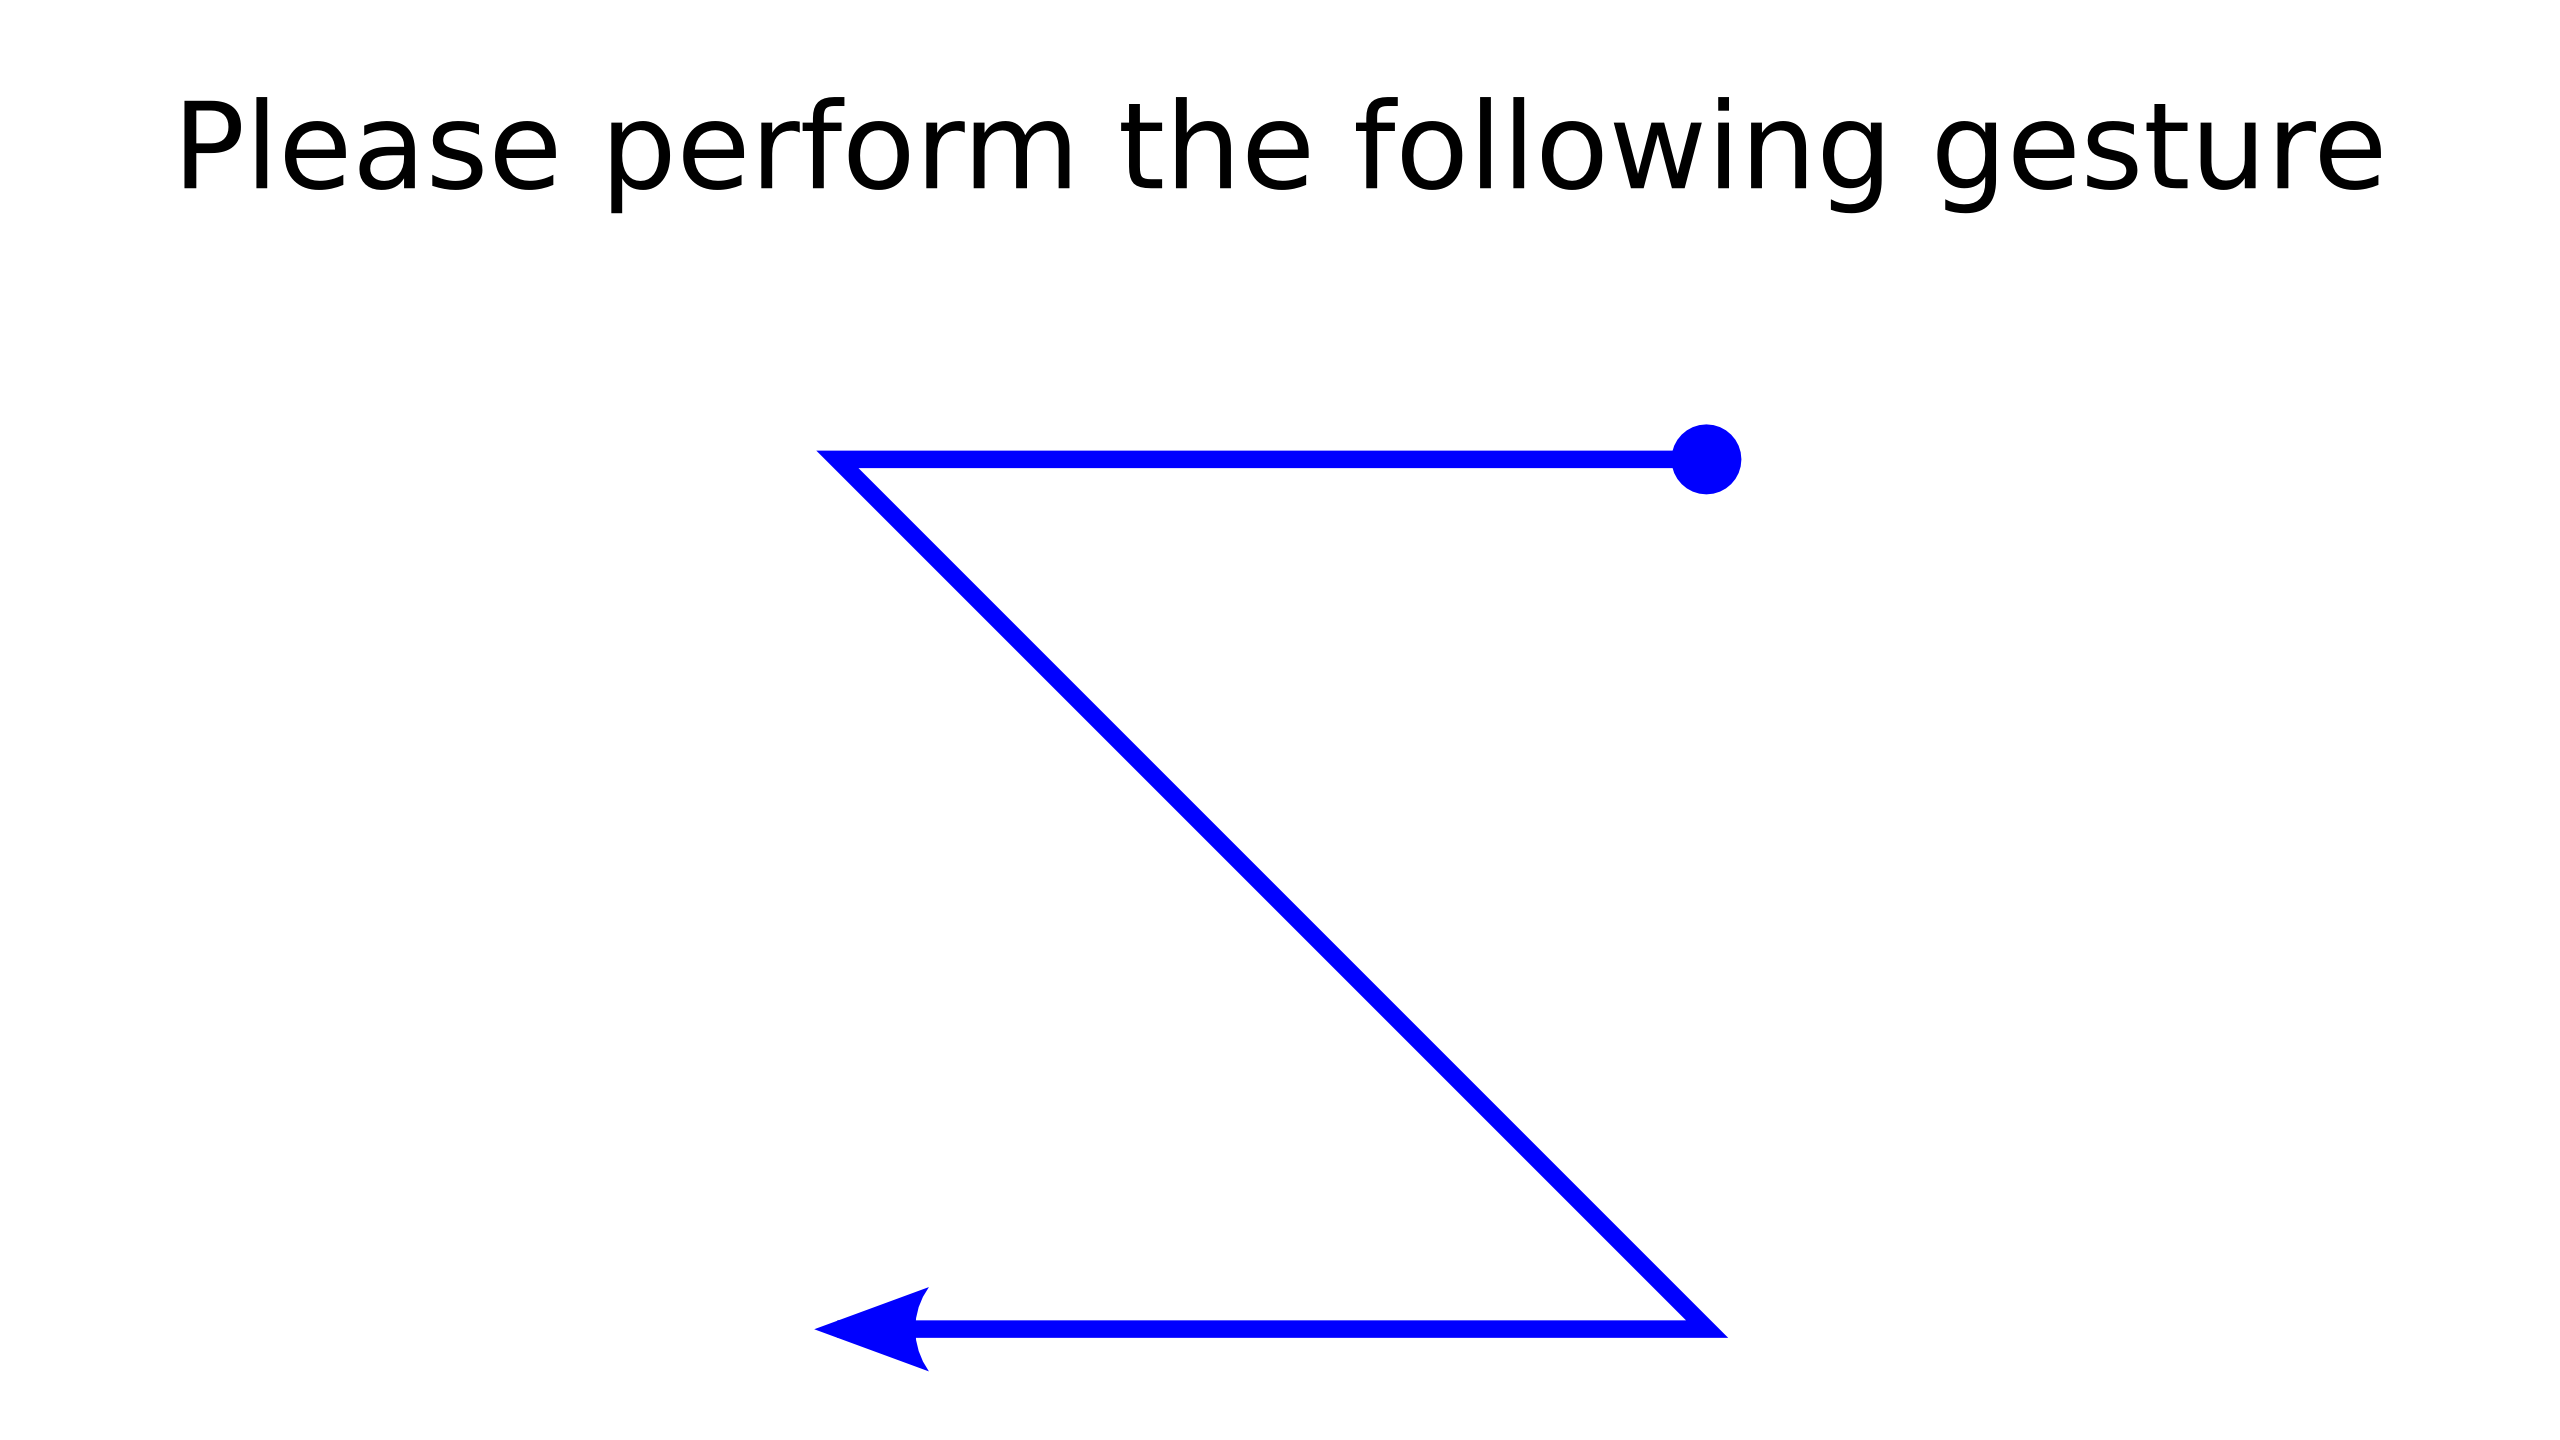
\includegraphics[width=0.25\textwidth]{3.png}} &
                \frame{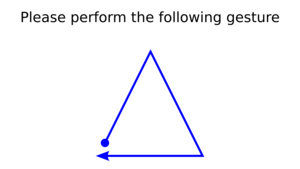
\includegraphics[width=0.25\textwidth]{4.png}} &
                \frame{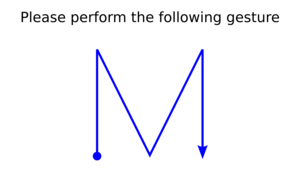
\includegraphics[width=0.25\textwidth]{5.png}} \\
                \frame{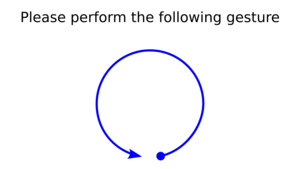
\includegraphics[width=0.25\textwidth]{6.png}} &
                \frame{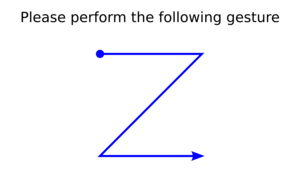
\includegraphics[width=0.25\textwidth]{7.png}} &
                \frame{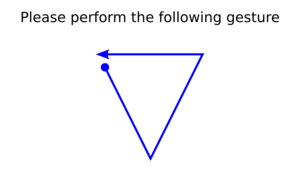
\includegraphics[width=0.25\textwidth]{8.png}} &
                \frame{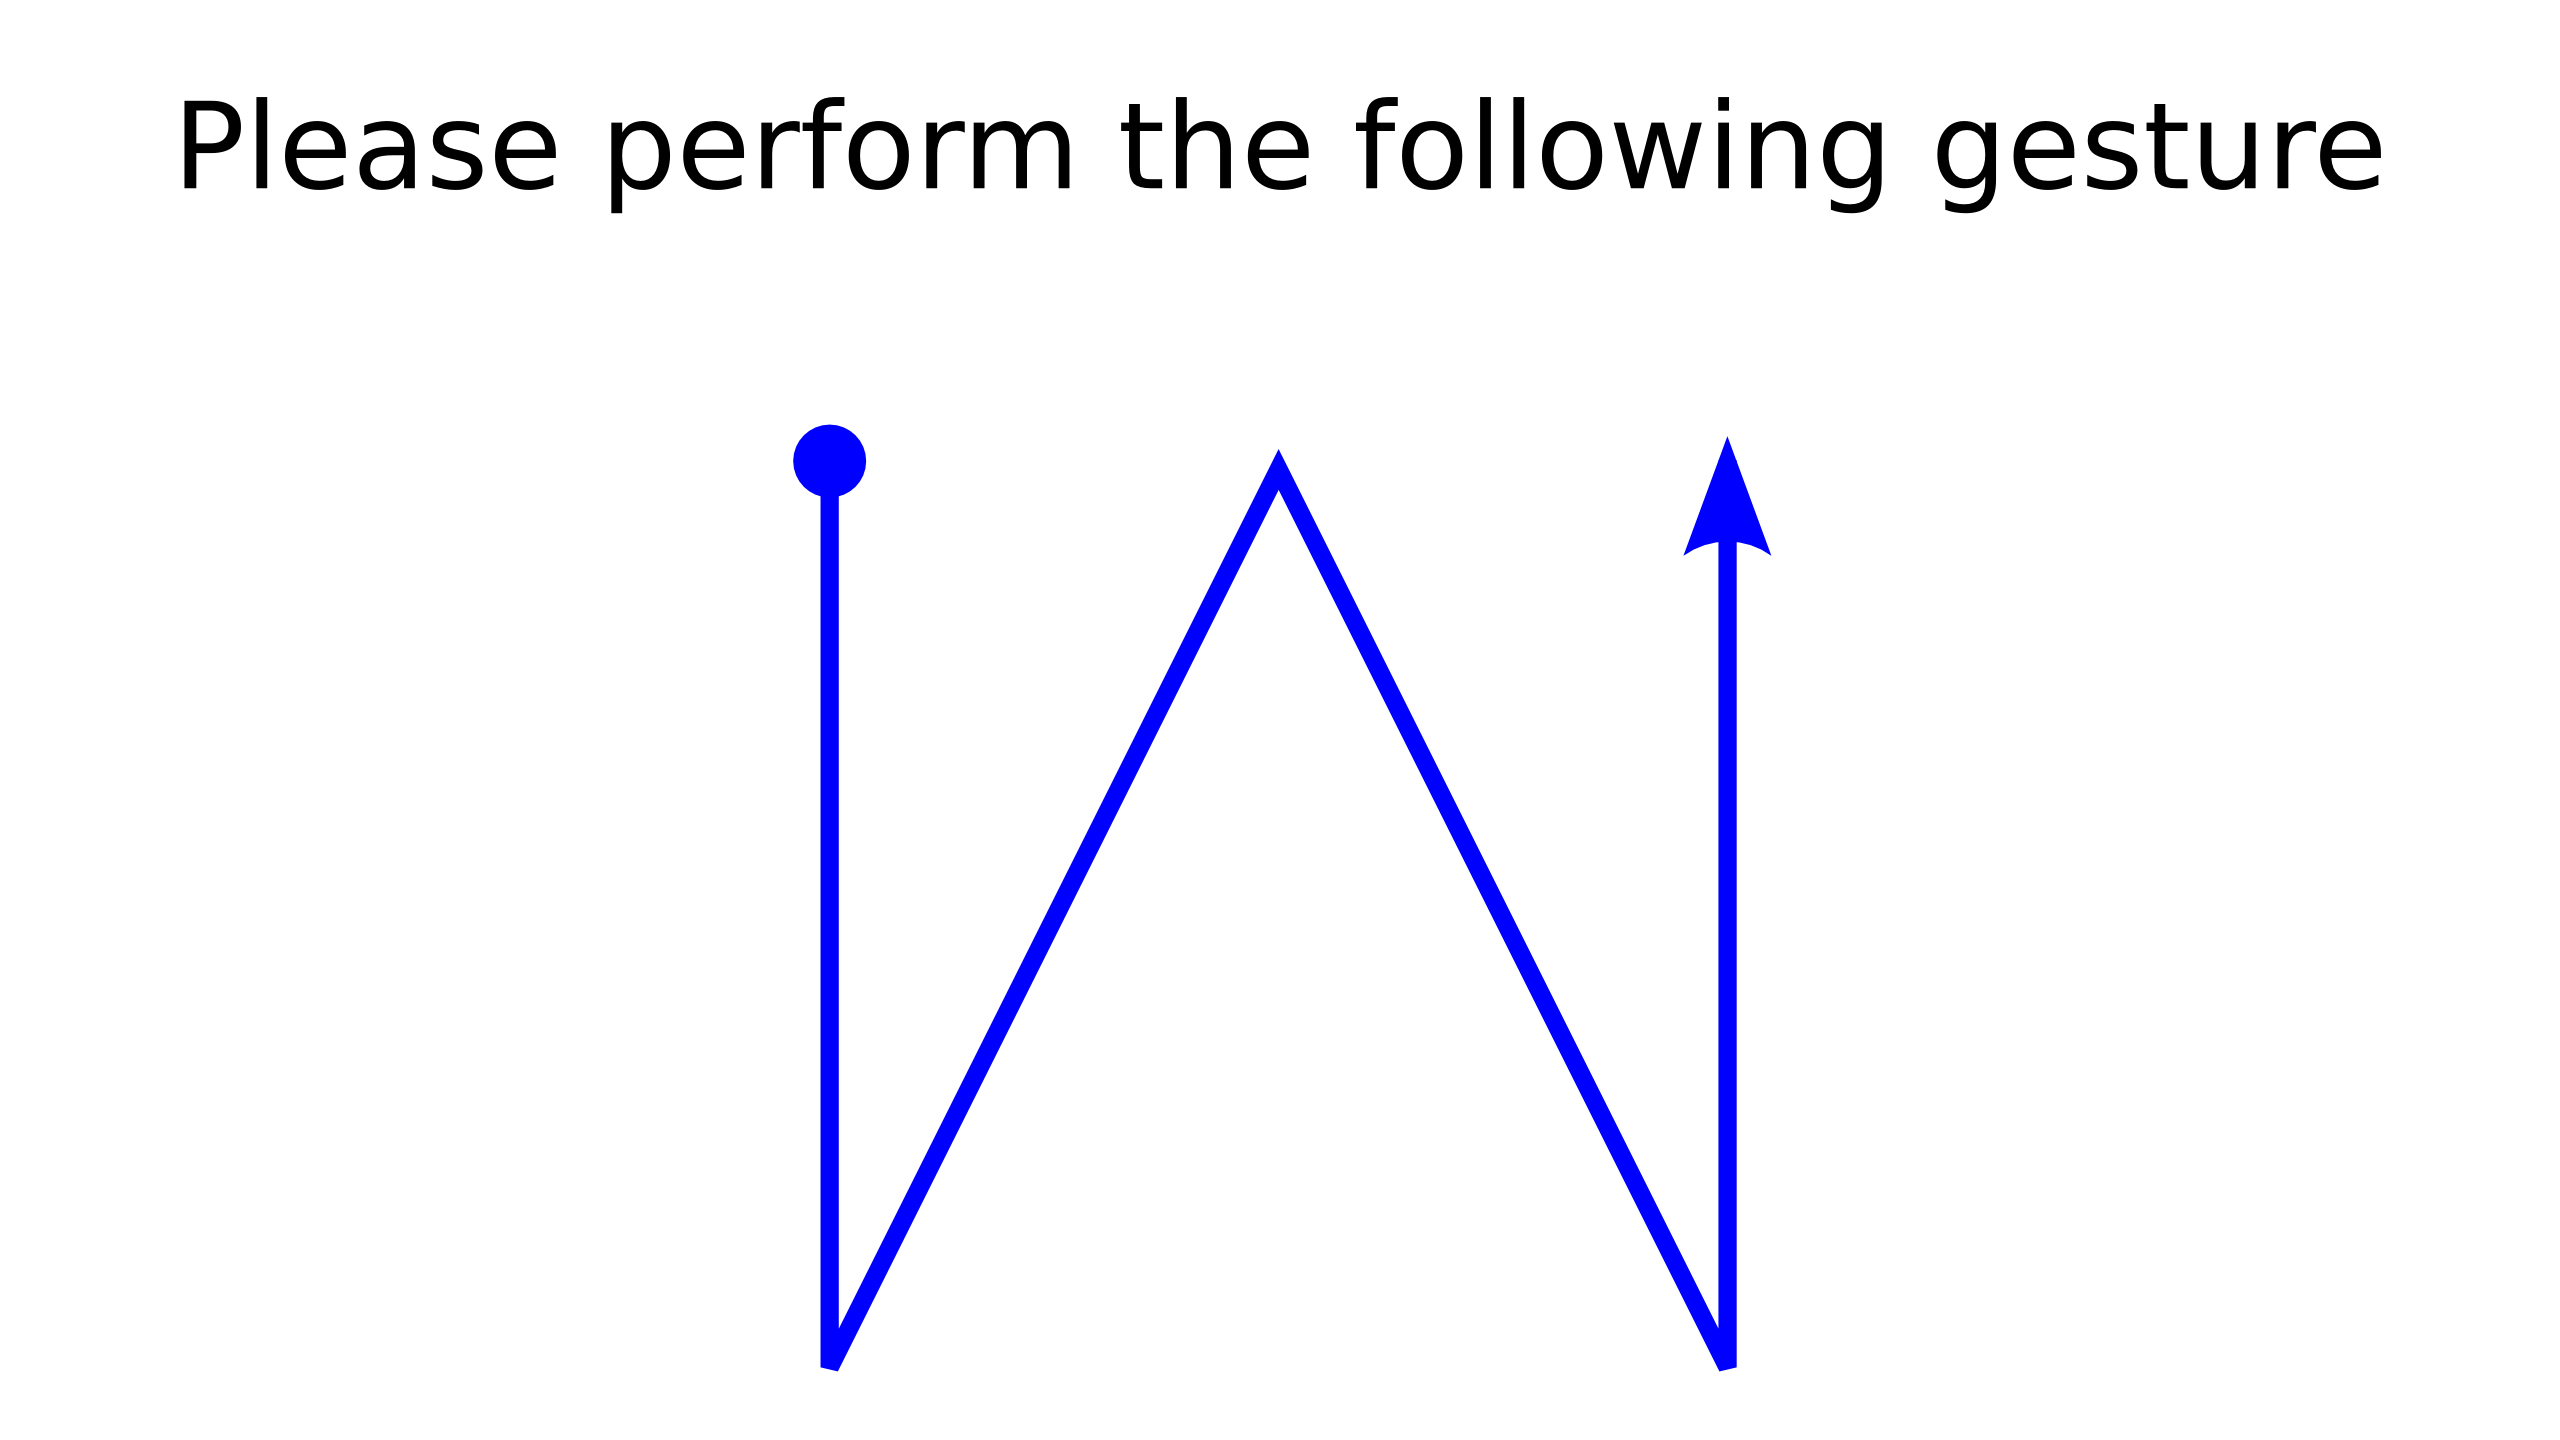
\includegraphics[width=0.25\textwidth]{9.png}} &
                \frame{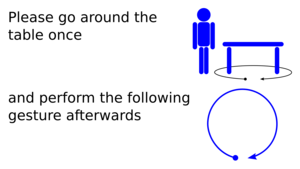
\includegraphics[width=0.25\textwidth]{10.png}} \\
                \frame{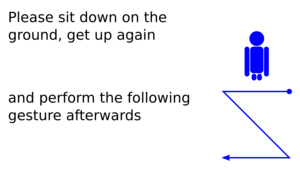
\includegraphics[width=0.25\textwidth]{11.png}} &
                \frame{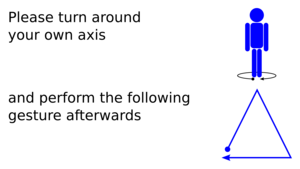
\includegraphics[width=0.25\textwidth]{12.png}} &
                \frame{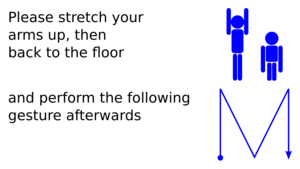
\includegraphics[width=0.25\textwidth]{13.png}} &
                \frame{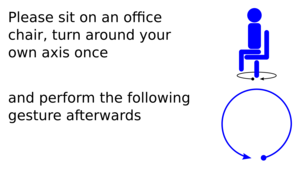
\includegraphics[width=0.25\textwidth]{14.png}} &
                \frame{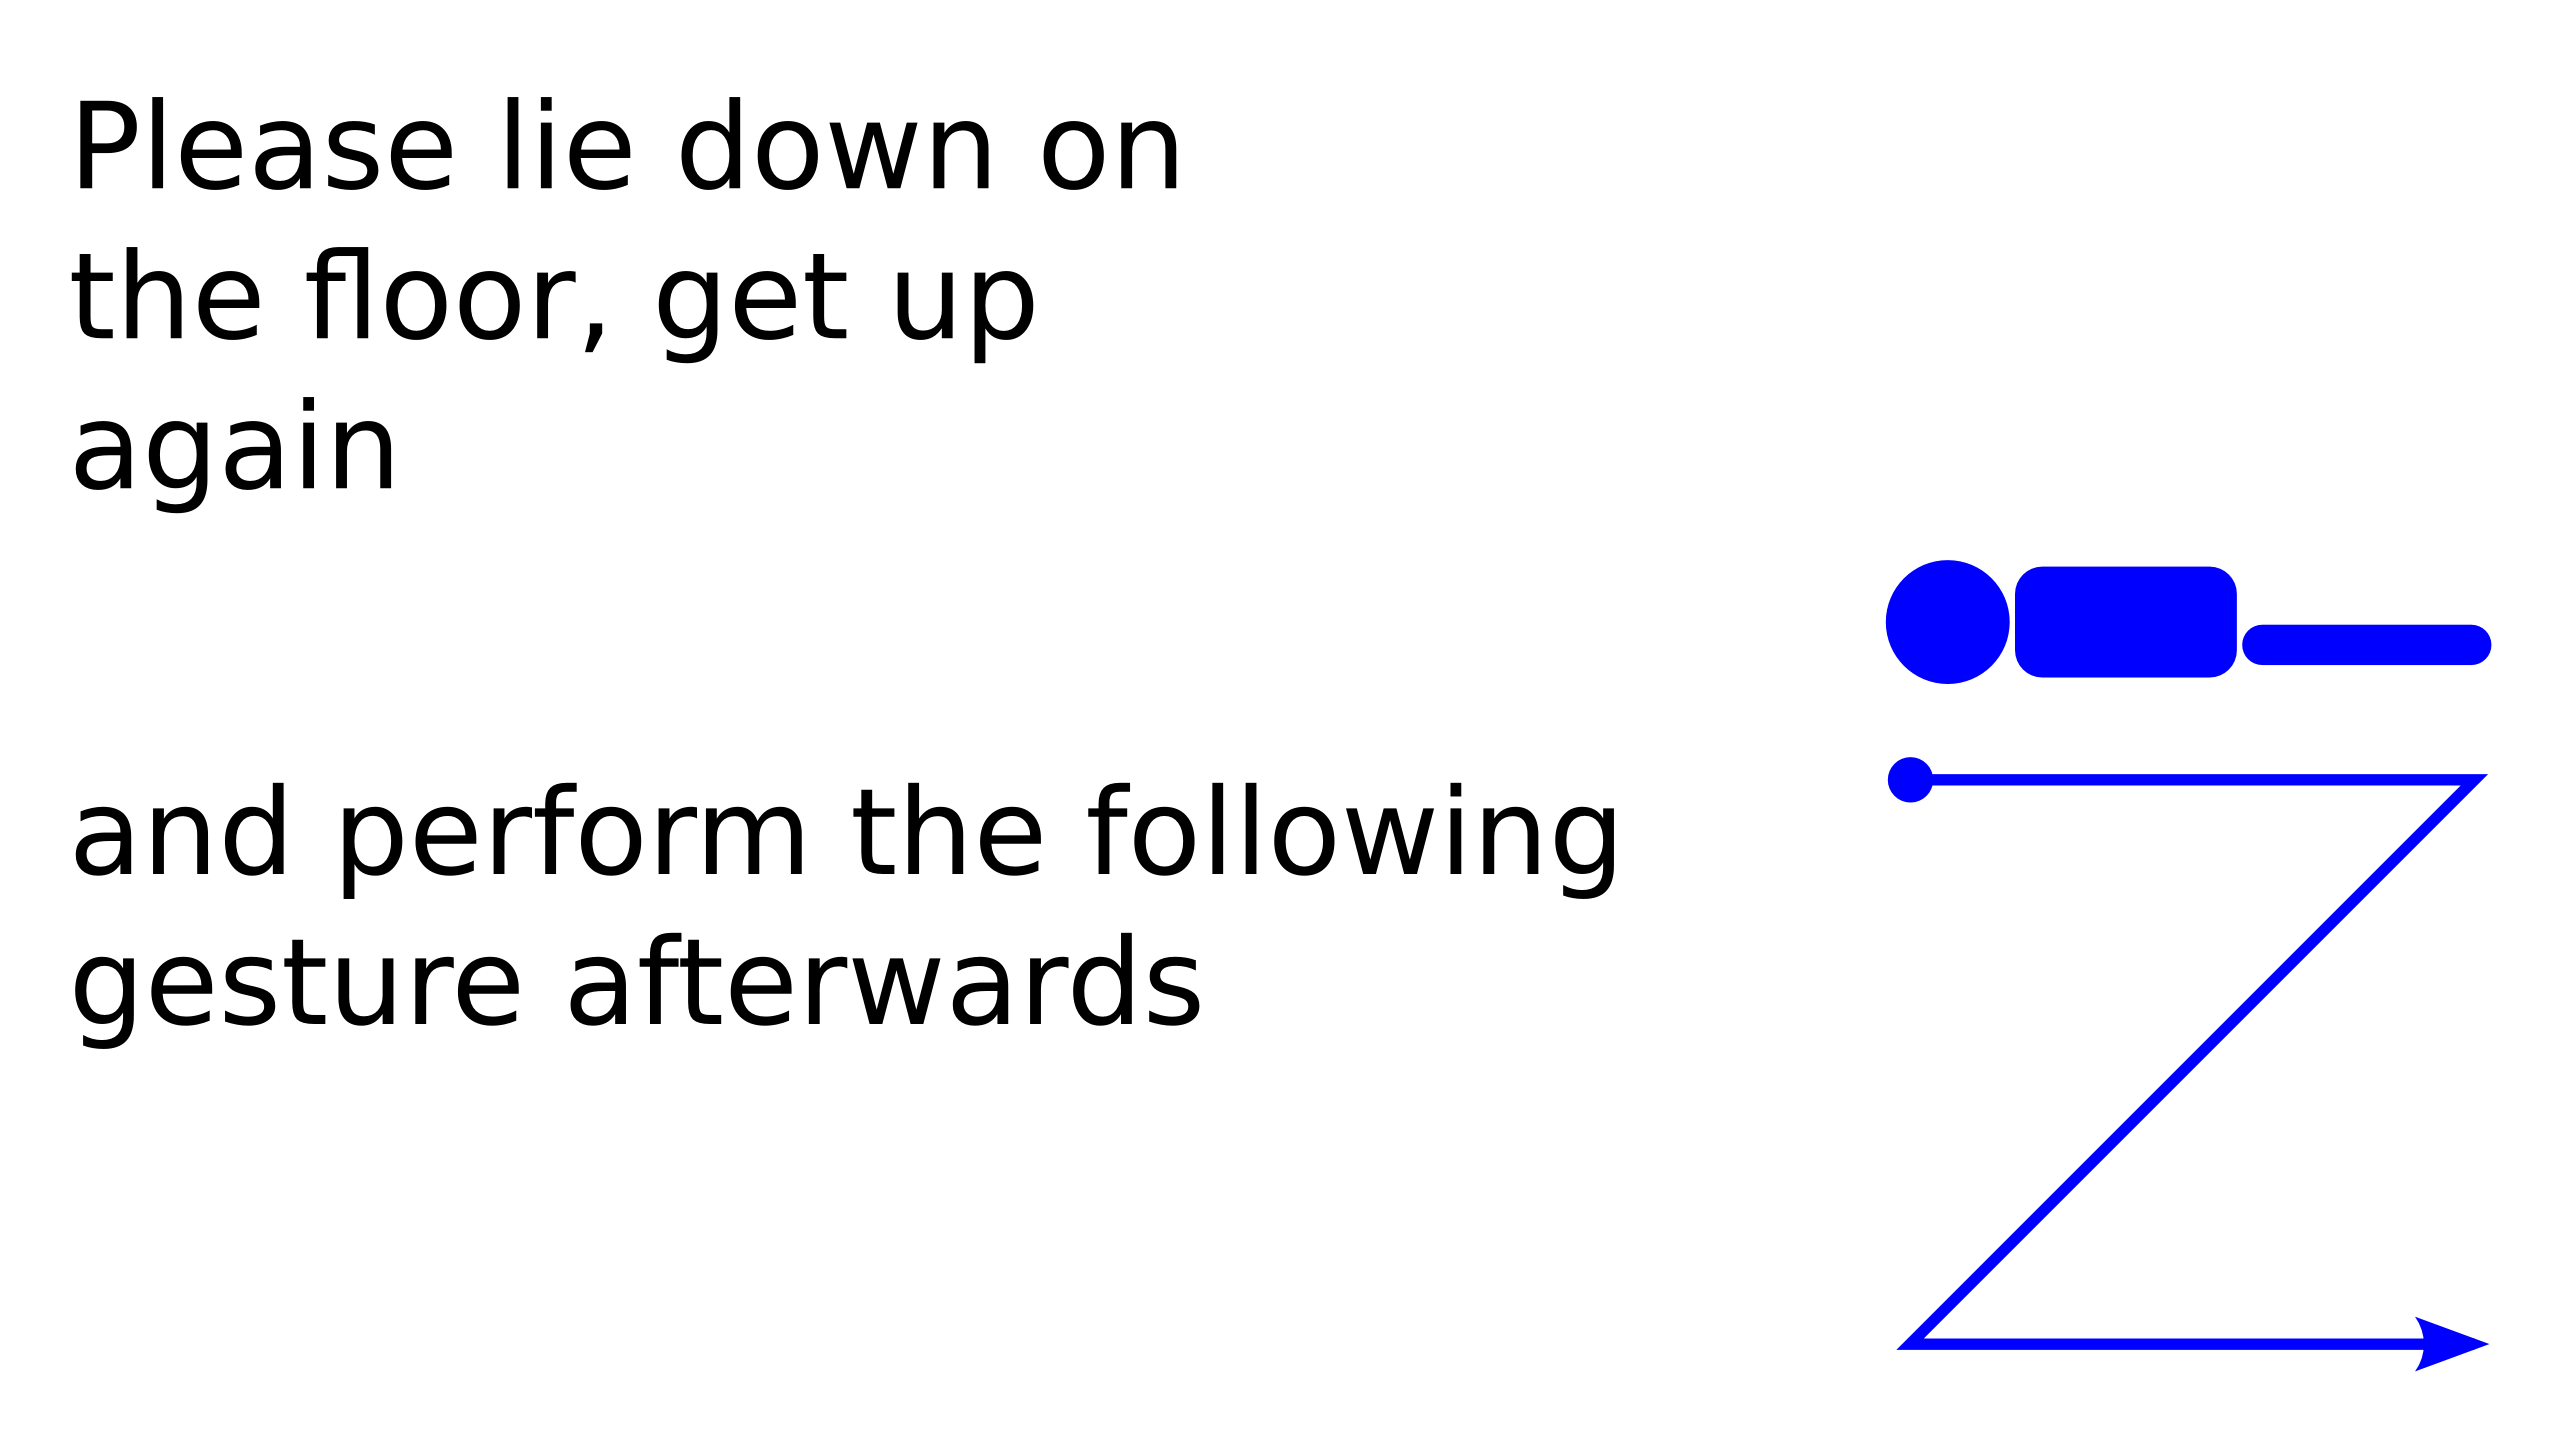
\includegraphics[width=0.25\textwidth]{15.png}} \\
                \frame{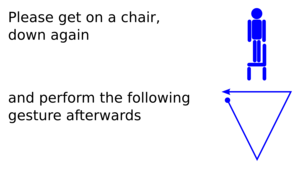
\includegraphics[width=0.25\textwidth]{16.png}} &
                \frame{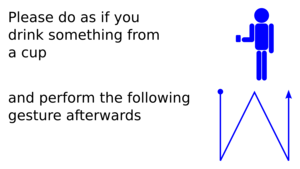
\includegraphics[width=0.25\textwidth]{17.png}} &
                \frame{
\includegraphics[width=0.25\textwidth]{18.png}} &
                \frame{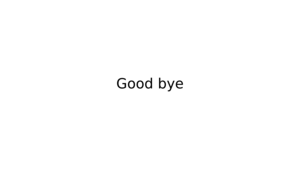
\includegraphics[width=0.25\textwidth]{19.png}} \\
            \end{tabular}
        }
    \end{center}
\end{frame}

\begin{frame}{Evaluation}{Recording Example}
    \resizebox {\textwidth} {!} {
        \begin{tikzpicture}
            \begin{axis}[
                xmin=0,
                xmax=3176,
                ymin=-16,
                ymax=16,
                width=10*\axisdefaultwidth,
                height=\axisdefaultheight,
                xticklabels={,,},
                yticklabels={,,}]
                \addplot[blue, mark=none, opacity=0.4] table[x=t, y=x] {../data/fig/record1/timeseries.dat};
                \addplot[red, mark=none, opacity=0.4] table[x=t, y=y] {../data/fig/record1/timeseries.dat};
                \addplot[green, mark=none, opacity=0.4] table[x=t, y=z] {../data/fig/record1/timeseries.dat};
                \addplot+[fill, opacity=0.5, blue, mark=none] coordinates {(38, -16) (89, -16) (89, 16) (38, 16)} --cycle;
                \addplot+[fill, opacity=0.5, blue, mark=none] coordinates {(123, -16) (177, -16) (177, 16) (123, 16)} --cycle;
                \addplot+[fill, opacity=0.5, blue, mark=none] coordinates {(201, -16) (256, -16) (256, 16) (201, 16)} --cycle;
                \addplot+[fill, opacity=0.5, blue, mark=none] coordinates {(282, -16) (355, -16) (355, 16) (282, 16)} --cycle;
                \addplot+[fill, opacity=0.5, blue, mark=none] coordinates {(388, -16) (439, -16) (439, 16) (388, 16)} --cycle;
                \addplot+[fill, opacity=0.5, blue, mark=none] coordinates {(473, -16) (530, -16) (530, 16) (473, 16)} --cycle;
                \addplot+[fill, opacity=0.5, blue, mark=none] coordinates {(568, -16) (624, -16) (624, 16) (568, 16)} --cycle;
                \addplot+[fill, opacity=0.5, blue, mark=none] coordinates {(672, -16) (749, -16) (749, 16) (672, 16)} --cycle;
                \addplot+[fill, opacity=0.5, blue, mark=none] coordinates {(1057, -16) (1106, -16) (1106, 16) (1057, 16)} --cycle;
                \addplot+[fill, opacity=0.5, blue, mark=none] coordinates {(1258, -16) (1313, -16) (1313, 16) (1258, 16)} --cycle;
                \addplot+[fill, opacity=0.5, blue, mark=none] coordinates {(1472, -16) (1527, -16) (1527, 16) (1472, 16)} --cycle;
                \addplot+[fill, opacity=0.5, blue, mark=none] coordinates {(1690, -16) (1772, -16) (1772, 16) (1690, 16)} --cycle;
                \addplot+[fill, opacity=0.5, blue, mark=none] coordinates {(2066, -16) (2116, -16) (2116, 16) (2066, 16)} --cycle;
                \addplot+[fill, opacity=0.5, blue, mark=none] coordinates {(2439, -16) (2497, -16) (2497, 16) (2439, 16)} --cycle;
                \addplot+[fill, opacity=0.5, blue, mark=none] coordinates {(2840, -16) (2895, -16) (2895, 16) (2840, 16)} --cycle;
                \addplot+[fill, opacity=0.5, blue, mark=none] coordinates {(3061, -16) (3137, -16) (3137, 16) (3061, 16)} --cycle;
            \end{axis}
        \end{tikzpicture}
    }
\end{frame}

\begin{frame}{Evaluation}{Data Preparation}
    \begin{itemize}
        \item \textit{Resampling}: data was resampled by means of the moving average technique, using a window size of 50 ms and step size of 30 ms
        \item \textit{Quantization}: converted into time series with integer values between -16 and 16, such as suggested in related work \cite{liu2009uwave}\\
        \begin{center}
            \tiny
            \begin{tabular}{cc}
                \hline
                \textbf{Acceleration data ($a$) in $\frac{dm}{s^2}$} & \textbf{Converted value}\\
                \hline
                $a > 200$ & 16\\
                $100 < a < 200$ & 11 to 15 (five levels linearly)\\
                $0 < a < 100$ & 1 to 10 (ten levels linearly)\\
                $a = 0$ & 0\\
                $-100 < a < 0$ & -1 to - 10 (ten levels linearly)\\
                $-200 < a < -100$ & -11 to - 15 (five levels linearly)\\
                $a < -200$ & -16\\
                \hline
            \end{tabular}
        \end{center}
    \end{itemize}
\end{frame}

\begin{frame}{Evaluation}{Data Preparation Example}
    \begin{center}
        \resizebox {\textwidth} {!} {
            \begin{tabular}{ccc}
                \resizebox {!} {\height} {
                    \begin{tikzpicture}
                        \begin{axis}[
                            xmin=1,
                            xmax=295,
                            xlabel=time,
                            ylabel=acceleration in $\frac{dm}{s^2}$]
                            \addplot[blue, ultra thick, mark=none] table[x=t, y=x] {../data/fig/quantization/raw.dat};
                            \addplot[red, ultra thick, mark=none] table[x=t, y=y] {../data/fig/quantization/raw.dat};
                            \addplot[green, ultra thick, mark=none] table[x=t, y=z] {../data/fig/quantization/raw.dat};
                        \end{axis}
                    \end{tikzpicture}
                } &
                \resizebox {!} {\height} {
                    \begin{tikzpicture}
                        \pgfplotsset{every axis legend/.append style={
                    		at={(0.5,1.03)},
                    		anchor=south}}
                        \begin{axis}[
                            xmin=1,
                            xmax=52,
                            xlabel=time,
                            ylabel=acceleration in $\frac{dm}{s^2}$,
                            legend columns=4]
                            \addplot[blue, ultra thick, mark=none] table[x=t, y=x] {../data/fig/quantization/compressed.dat};
                            \addlegendentry{x-axis}
                            \addplot[red, ultra thick, mark=none] table[x=t, y=y] {../data/fig/quantization/compressed.dat};
                            \addlegendentry{y-axis}
                            \addplot[green, ultra thick, mark=none] table[x=t, y=z] {../data/fig/quantization/compressed.dat};
                            \addlegendentry{z-axis}
                        \end{axis}
                    \end{tikzpicture}
                } &
                \resizebox {!} {\height} {
                    \begin{tikzpicture}
                        \begin{axis}[
                            xmin=1,
                            xmax=52,
                            xlabel=time,
                            ylabel=converted acceleration]
                            \addplot[blue, ultra thick, mark=none] table[x=t, y=x] {../data/fig/quantization/converted.dat};
                            \addplot[red, ultra thick, mark=none] table[x=t, y=y] {../data/fig/quantization/converted.dat};
                            \addplot[green, ultra thick, mark=none] table[x=t, y=z] {../data/fig/quantization/converted.dat};
                        \end{axis}
                    \end{tikzpicture}
                }
            \end{tabular}
        }
    \end{center}
\end{frame}

\begin{frame}{Experiment}{Model parameters}
    \begin{itemize}
        \item \textit{window size}: determines the number of most recent measurements
            \begin{itemize}
                \item min
                \item max
                \item avg
                \item mid
            \end{itemize}
        \item \textit{step size}: defines the gap between consecutive time series windows
            \begin{itemize}
                \item tenth of the window size
            \end{itemize}
        \item \textit{normalization}: normalization prior to pair-wise comparing sliding windows and training gestures
            \begin{itemize}
                \item $\eta$ normalization
                \item $z$ normalization
                \item no normalization
            \end{itemize}
    \end{itemize}
\end{frame}

\begin{frame}{Experiment}{Model Parameters}
    \begin{itemize}
        \item \textit{Sakoe-Chiba band sizes}:
            \begin{itemize}
                \item 34 different between 1 \% to 100 \%
            \end{itemize}
        \item \textit{threshold}: defines the time series distance at which a sliding window and a training gesture are considered to belong to the same class
            \begin{itemize}
                \item HMinD
                \item HAvgD
                \item HMidD
            \end{itemize}
        \item \textit{filter criterion}:
            \begin{itemize}
                \item VAR
                \item LNCE
                \item no filter
            \end{itemize}
    \end{itemize}
\end{frame}

\begin{frame}{Experiment}{Example Result}
    \resizebox {\textwidth} {!} {
        \begin{tikzpicture}
            \begin{axis}[
                xmin=0,
                xmax=2426,
                ymin=-16,
                ymax=16,
                width=10*\axisdefaultwidth,
                height=\axisdefaultheight,
                xticklabels={,,},
                yticklabels={,,}]
                \addplot[blue, mark=none, opacity=0.4] table[x=t, y=x] {../data/fig/experimentee_result2/exp1.dat};
                \addplot[red, mark=none, opacity=0.4] table[x=t, y=y] {../data/fig/experimentee_result2/exp1.dat};
                \addplot[green, mark=none, opacity=0.4] table[x=t, y=z] {../data/fig/experimentee_result2/exp1.dat};
                \addplot+[fill, opacity=0.5, red, mark=none] coordinates {(294, -16) (307, -16) (307, 16) (294, 16)} --cycle;
                \addplot+[fill, opacity=0.5, green, mark=none] coordinates {(307, -16) (357, -16) (357, 16) (307, 16)} --cycle;
                \addplot+[fill, opacity=0.5, red, mark=none] coordinates {(357, -16) (359, -16) (359, 16) (357, 16)} --cycle;
                \addplot+[fill, opacity=0.5, red, mark=none] coordinates {(497, -16) (508, -16) (508, 16) (497, 16)} --cycle;
                \addplot+[fill, opacity=0.5, green, mark=none] coordinates {(508, -16) (562, -16) (562, 16) (508, 16)} --cycle;
                \addplot+[fill, opacity=0.5, blue, mark=none] coordinates {(562, -16) (564, -16) (564, 16) (562, 16)} --cycle;
                \addplot+[fill, opacity=0.5, red, mark=none] coordinates {(712, -16) (722, -16) (722, 16) (712, 16)} --cycle;
                \addplot+[fill, opacity=0.5, green, mark=none] coordinates {(722, -16) (777, -16) (777, 16) (722, 16)} --cycle;
                \addplot+[fill, opacity=0.5, blue, mark=none] coordinates {(777, -16) (778, -16) (778, 16) (777, 16)} --cycle;
                \addplot+[fill, opacity=0.5, blue, mark=none] coordinates {(940, -16) (945, -16) (945, 16) (940, 16)} --cycle;
                \addplot+[fill, opacity=0.5, green, mark=none] coordinates {(945, -16) (1010, -16) (1010, 16) (945, 16)} --cycle;
                \addplot+[fill, opacity=0.5, blue, mark=none] coordinates {(1010, -16) (1023, -16) (1023, 16) (1010, 16)} --cycle;
                \addplot+[fill, opacity=0.5, red, mark=none] coordinates {(1310, -16) (1316, -16) (1316, 16) (1310, 16)} --cycle;
                \addplot+[fill, opacity=0.5, green, mark=none] coordinates {(1316, -16) (1367, -16) (1367, 16) (1316, 16)} --cycle;
                \addplot+[fill, opacity=0.5, red, mark=none] coordinates {(1367, -16) (1375, -16) (1375, 16) (1367, 16)} --cycle;
                \addplot+[fill, opacity=0.5, red, mark=none] coordinates {(1681, -16) (1689, -16) (1689, 16) (1681, 16)} --cycle;
                \addplot+[fill, opacity=0.5, green, mark=none] coordinates {(1689, -16) (1746, -16) (1746, 16) (1689, 16)} --cycle;
                \addplot+[fill, opacity=0.5, blue, mark=none] coordinates {(1746, -16) (1748, -16) (1748, 16) (1746, 16)} --cycle;
                \addplot+[fill, opacity=0.5, red, mark=none] coordinates {(2082, -16) (2090, -16) (2090, 16) (2082, 16)} --cycle;
                \addplot+[fill, opacity=0.5, green, mark=none] coordinates {(2090, -16) (2146, -16) (2146, 16) (2090, 16)} --cycle;
                \addplot+[fill, opacity=0.5, red, mark=none] coordinates {(2146, -16) (2147, -16) (2147, 16) (2146, 16)} --cycle;
                \addplot+[fill, opacity=0.5, blue, mark=none] coordinates {(2311, -16) (2388, -16) (2388, 16) (2311, 16)} --cycle;
                \addplot+[fill, opacity=0.5, red, mark=none] coordinates {(2297, -16) (2362, -16) (2362, 16) (2297, 16)} --cycle;
            \end{axis}
        \end{tikzpicture}
    }
\end{frame}

\begin{frame}{Performance Measures}
        $Precision_{\mu} = {\sum \limits_{i=1}^{l} tp_i}  \bigg/  {\sum \limits_{i=1}^{l} (tp_i + fp_i)}$\\
        $Recall_{\mu} = {\sum \limits_{i=1}^{l} tp_i} \bigg/{\sum \limits_{i=1}^{l} (tp_i + fn_i)}$\\
        $F_{\beta}score_{\mu} = {(\beta^2 + 1)Precision_{\mu} Recall_{\mu}} \bigg/ {\beta^2 Precision_{\mu} + Recall_{\mu}}$\\
\end{frame}

\begin{frame}{Evaluation}{Simulations ranked by $F_{1}score_{\mu}$}
    \begin{center}
        \resizebox {0.5\textwidth} {!} {
            \begin{tikzpicture}[spy using outlines={circle, magnification=6, connect spies}]
                \begin{axis}[
                    xmin=0,
                    xmax=1,
                    ymin=0,
                    ymax=1,
                    width=\axisdefaultwidth,
                    height=\axisdefaultwidth,
                    xlabel=$Precision_{\mu}$,
                    ylabel=$Recall_{\mu}$,
                    samples=100,
                    colorbar horizontal,
                    colormap/viridis high res,
                    title=$F_{1}score_{\mu}$]
                    \addplot[only marks, scatter, scatter src=explicit, mark size=1] table[x=x,y=y,meta=fscore] {../data/fig/result2/result.dat};
                    \addplot[gray, domain=0.051:1] {(0.1 * x) / (2 * x - 0.1)};
                    \addplot[gray, domain=0.11:1] {(0.2 * x) / (2 * x - 0.2)};
                    \addplot[gray, domain=0.16:1] {(0.3 * x) / (2 * x - 0.3)};
                    \addplot[gray, domain=0.21:1] {(0.4 * x) / (2 * x - 0.4)};
                    \addplot[gray, domain=0.26:1] {(0.5 * x) / (2 * x - 0.5)};
                    \addplot[gray, domain=0.31:1] {(0.6 * x) / (2 * x - 0.6)};
                    \addplot[gray, domain=0.36:1] {(0.7 * x) / (2 * x - 0.7)};
                    \addplot[gray, domain=0.41:1] {(0.8 * x) / (2 * x - 0.8)};
                    \addplot[gray, domain=0.46:1] {(0.9 * x) / (2 * x - 0.9)};
                    \coordinate (spypoint) at (axis cs:0.8413867433,0.6578651685);
                    \coordinate (magnifyglass) at (axis cs:0.2,0.8);
                \end{axis}
                \spy [size=2cm] on (spypoint)
                    in node[fill=white] at (magnifyglass);
            \end{tikzpicture}
        }
    \end{center}
\end{frame}


    \newpage
\section{Conclusion and Future Work} \label{conclusion_and_future_work}

- Summaries results
- Implications
- Possibilities and potential applications
    \clearpage
    \begin{thebibliography}{1}
    \bibitem{xi2006fast} Xi, Xiaopeng and Keogh, Eamonn and Shelton, Christian and Wei, Li and Ratanamahatana, Chotirat
    Ann "Fast time series classification using numerosity reduction" Proceedings of the 23rd international conference on
    Machine learning (2006): 1033--1040
    \bibitem{ding2008querying} Ding, Hui and Trajcevski, Goce and Scheuermann, Peter and Wang, Xiaoyue and Keogh, Eamonn
    "Querying and mining of time series data: experimental comparison of representations and distance measures"
    Proceedings of the VLDB Endowment (2008): 1542--1552.
    \bibitem{keogh2002exact} Keogh, Eamonn "Exact indexing of dynamic time warping" Proceedings of the 28th
    international conference on Very Large Data Bases (2002): 406--417
    \bibitem{berndt1994using} Berndt, Donald J and Clifford, James "Using dynamic time warping to find patterns in time
    series." KDD workshop (1994): 359--370
    \bibitem{batista2011complexity} Batista, Gustavo EAPA and Wang, Xiaoyue and Keogh, Eamonn J "A
    Complexity-Invariant Distance Measure for Time Series." SDM (2011): 699--710
    \bibitem{liu2009uwave} Liu, Jiayang and Zhong, Lin and Wickramasuriya, Jehan and Vasudevan, Venu "uWave:
    Accelerometer-based personalized gesture recognition and its applications" Pervasive and Mobile Computing
    (2009): 657--675
\end{thebibliography}

    \clearpage
    \section*{Zusammenfassung} \addcontentsline{toc}{section}{Attachment Zusammenfassung}
Viele unterschiedliche Ger\"ate im Leben des modernen Menschen produzieren untentwegt
Daten in den verschiedenesten Formen. Offensichtliche Beispiele daf\"ur sind intelligente Mobiltelefone, tragbare
Ger\"ate wie intelligente Uhren oder Titnessarmb\"ander. Ein betr\"achtlicher Anteil der Daten wird ununterbrochen
produziert und kann als Zeitreihendatenstrom interpretiert werden. Zum Beispiel Beschleunigungs- oder
Vitalit\"atsdaten. Eine Echtzeitanalyse dieses Zeitreihendatenstroms bedingt m\"oglicher Weise eine konstant
ausgef\"uhrte Erster-N\"achster-Nachbar (1NN) Klassifizierung auf dem aktuellen Zeitreihenfenster mit einem
Distanzma{\ss} wie Dynamic Time Warping (DTW). Die begrenzten Mittel von tragbaren Ger\"aten oder Mikrocontrollern
zwingen zu einem sparsamen Umgang mit Speicher und Laufzeit.

Diese Bachelorarbeit erkl\"art den Ansatz eines Filters f\"ur Zeitreihen mit linearer Komplexit\"at vor 1NN-DTW. Der
Mehrwert eines Filters mit geringer Laufzeit ist dabei die Einsparung von kostenintensiven 1NN-DTW Ausf\"uhrungen im
Falle von nicht klassifizierbaren Zeitreihenfenstern. Anhand von Ergebnissen eines beispielhaften Experiments mit
Gestenerkennung durch Beschleunigungsdaten wird gezeigt, dass Filter mit nur geringem Genauigkeitsverlust die
Ausf\"uhrung von 1NN-DTW reduzieren k\"onnen.

\end{document}
